% !TeX document-id = {76546e66-bdd4-43d8-b74c-0b64d126e97d}
% !TEX TS-program = XeLaTeX
% use the following command:
% all document files must be coded in UTF-8
\documentclass[portuguese]{textolivre}
% build HTML with: make4ht -e build.lua -c textolivre.cfg -x -u article "fn-in,svg,pic-align"

\journalname{Texto Livre}
\thevolume{18}
%\thenumber{1} % old template
\theyear{2025}
\receiveddate{\DTMdisplaydate{2024}{1}{25}{-1}} % YYYY MM DD
\accepteddate{\DTMdisplaydate{2024}{10}{16}{-1}}
\publisheddate{\today}
\corrauthor{Rafael Oliveira Vasconcelos}
\articledoi{10.35699/1983-3652.2025.50815}
%\articleid{NNNN} % if the article ID is not the last 5 numbers of its DOI, provide it using \articleid{} commmand 
% list of available sesscions in the journal: articles, dossier, reports, essays, reviews, interviews, editorial
\articlesessionname{articles}

%apagar
\runningauthor{Neto e Vasconcelos} 
%descomentar


%\editorname{Leonardo Araújo} % old template
\sectioneditorname{Daniervelin Pereira}
\layouteditorname{Leonardo Araújo}

\title{Proposta de modelo para votação eletrônica utilizando Blockchain e Contratos Inteligentes}
\othertitle{Model proposal for electronic voting using Blockchain and Smart Contracts}
% if there is a third language title, add here:
%\othertitle{Artikelvorlage zur Einreichung beim Texto Livre Journal}

%apagar
\author[1]{José Alves de Lima Neto~\orcid{0009-0001-1324-9513}\thanks{Email: \href{mailto:jalneto@dcomp.ufs.br}{jalneto@dcomp.ufs.br}}}
\author[1]{Rafael Oliveira Vasconcelos ~\orcid{0000-0001-7974-304X}\thanks{Email: \href{mailto:rafael@dcomp.ufs.br}{rafael@dcomp.ufs.br}}}
\affil[1]{Universidade Federal de Sergipe, DComp, São Cristóvão, SE, Brasil.}


\addbibresource{article.bib}
% use biber instead of bibtex
% $ biber article

% used to create dummy text for the template file
%\definecolor{dark-gray}{gray}{0.35} % color used to display dummy texts
\usepackage{lipsum}
\SetLipsumParListSurrounders{\colorlet{oldcolor}{.}\color{dark-gray}}{\color{oldcolor}}

% used here only to provide the XeLaTeX and BibTeX logos
\usepackage{hologo}

% if you use multirows in a table, include the multirow package
%\usepackage{multirow}

% provides sidewaysfigure environment
%\usepackage{rotating}

% % CUSTOM EPIGRAPH - BEGIN 
% %%% https://tex.stackexchange.com/questions/193178/specific-epigraph-style
% \usepackage{epigraph}
% \renewcommand\textflush{flushright}
% \makeatletter
% \newlength\epitextskip
% \pretocmd{\@epitext}{\em}{}{}
% \apptocmd{\@epitext}{\em}{}{}
% \patchcmd{\epigraph}{\@epitext{#1}\\}{\@epitext{#1}\\[\epitextskip]}{}{}
% \makeatother
% \setlength\epigraphrule{0pt}
% \setlength\epitextskip{0.5ex}
% \setlength\epigraphwidth{.7\textwidth}
% % CUSTOM EPIGRAPH - END

% LANGUAGE - BEGIN
% ARABIC
% for languages that use special fonts, you must provide the typeface that will be used
% \setotherlanguage{arabic}
% \newfontfamily\arabicfont[Script=Arabic]{Amiri}
% \newfontfamily\arabicfontsf[Script=Arabic]{Amiri}
% \newfontfamily\arabicfonttt[Script=Arabic]{Amiri}
%
% in the article, to add arabic text use: \textlang{arabic}{ ... }
%
% RUSSIAN
% for russian text we also need to define fonts with support for Cyrillic script
% \usepackage{fontspec}
% \setotherlanguage{russian}
% \newfontfamily\cyrillicfont{Times New Roman}
% \newfontfamily\cyrillicfontsf{Times New Roman}[Script=Cyrillic]
% \newfontfamily\cyrillicfonttt{Times New Roman}[Script=Cyrillic]
%
% in the text use \begin{russian} ... \end{russian}
% LANGUAGE - END

% EMOJIS - BEGIN
% to use emoticons in your manuscript
% https://stackoverflow.com/questions/190145/how-to-insert-emoticons-in-latex/57076064
% using font Symbola, which has full support
% the font may be downloaded at:
% https://dn-works.com/ufas/
% add to preamble:
% \newfontfamily\Symbola{Symbola}
% in the text use:
% {\Symbola }
% EMOJIS - END

% LABEL REFERENCE TO DESCRIPTIVE LIST - BEGIN
% reference itens in a descriptive list using their labels instead of numbers
% insert the code below in the preambule:
%\makeatletter
%\let\orgdescriptionlabel\descriptionlabel
%\renewcommand*{\descriptionlabel}[1]{%
	%  \let\orglabel\label
	%  \let\label\@gobble
	%  \phantomsection
	%  \edef\@currentlabel{#1\unskip}%
	%  \let\label\orglabel
	%  \orgdescriptionlabel{#1}%
	%}
%\makeatother
%
% in your document, use as illustraded here:
%\begin{description}
%  \item[first\label{itm1}] this is only an example;
%  % ...  add more items
%\end{description}
% LABEL REFERENCE TO DESCRIPTIVE LIST - END


% add line numbers for submission
%\usepackage{lineno}
%\linenumbers

\usepackage{xcolor} %Destacar fundo em amarelo
%\colorbox{yellow}{destacado com fundo amarelo}

\usepackage{soul} % Pacote para destacar texto
%\hl{um texto destacado em amarelo usando o comando hl do pacote soul}

\usepackage{array}
\usepackage{tabularx}
\usepackage{listings}

% Define a custom key "source" for lstlisting
\makeatletter
\lst@Key{source}\relax{} % Define a new key named "source"
\newcommand{\listingSource}{} % Create a command to store the source text
\lst@AddToHook{OnEmptyLine}{\def\listingSource{\lst@source}} % Store the value of the "source" key
\makeatother


\begin{document}
	\maketitle
	
	\begin{polyabstract}
		
		\begin{portuguese}
			\begin{abstract}
				As eleições para escolha de representantes políticos são indiscutivelmente uma das mais importantes manifestações da democracia de uma nação e, por isso, também é um momento crítico e de intensa responsabilidade para aqueles que a operam. Por sua importância, é necessário que atenda vários princípios de segurança, integridade e transparência, os quais foram recentemente contestados no contexto das eleições brasileiras.
				Diante disto e da boa combinação das redes \textit{blockchain} como agente benéfico para reforçar esses princípios, aplicando o método de pesquisa exploratória, este trabalho apresenta um modelo que aplica blockchain nas eleições brasileiras. Por fim, foram realizados testes funcionais e não funcionais. Os testes funcionais validaram a integridade e segurança do sistema ao permitir a submissão e verificação de votos de forma descentralizada, enquanto os testes não funcionais mostraram o possível custo da adoção deste tecnologia na eleição brasileira. Esses resultados reforçam o potencial da tecnologia blockchain para aprimorar o processo eleitoral brasileiro.
				
				\keywords{Eleições brasileiras \sep Votação eletrônica \sep Urna eletrônica \sep Blockchain \sep Contrato inteligente}
			\end{abstract}
		\end{portuguese}
		
		% if there is another abstract, insert it here using the same scheme
		\begin{english}
			\begin{abstract}
				
				The election to choose political representatives is undoubtedly one of the most important manifestations of a nation's democracy and, therefore, it is also a critical moment and of intense responsibility for those who operate it. Due to its importance, it is necessary to comply with several principles of security, integrity and transparency, which were recently challenged in the context of Brazilian elections. Faced with this challenge and recognizing the favorable combination of blockchain networks as a beneficial agent to reinforce these principles, applying the exploratory research method, this work presents a model that applies blockchain in Brazilian elections. Finally, functional and non-functional tests were carried out. Functional tests validated the system's integrity and security by allowing decentralized submission and verification of votes, while non-functional tests revealed the potential costs of adopting this technology in Brazilian elections. These results highlight the potential of blockchain technology to enhance the Brazilian electoral process.
				
				
				
				
				
				\keywords{ Brazilian elections \sep Electronic voting \sep Electronic ballot box \sep Blockchain \sep Smart contract}
			\end{abstract}
		\end{english}
		
		
	\end{polyabstract}
	
	
	\section{Introdução}\label{Introdução}
	
	Com o avanço das tecnologias, é natural que elas sejam inseridas cada vez mais em diversos cenários com o intuito de proporcionar melhorias, comodidade e segurança. Com o sistema eleitoral brasileiro não foi diferente. Com o principal intuito de trazer transparência e agilidade na apuração das eleições brasileiras, o sistema eleitoral brasileiro fez o uso de diversos recursos para gerir os processos de eleições federais, estaduais e municipais, que culminaram no uso das urnas eletrônicas \cite{sepulvida2019estudo}. Entretanto, existe uma recorrência acerca da confiabilidade no processo eleitoral \cite{machado2021vulnerabilidade}. 
	
	%Além disso, estes movimentos são reforçados pela tecnologia implementada no modelo atual, que segundo \textcite{picchia} apud \textcite{sepulvida2019estudo}, o tipo das urnas utilizadas no Brasil são da primeira geração dos equipamentos conhecidos como DRE (\textit{Direct Recording Electronic machine}), que utiliza método de salvamento sem segurança ou criptografia, cujo maior problema é a impossibilidade de auditoria. Embora tenha sido utilizada em outros países, esta geração foi descontinuada justamente por falta de confiabilidade nos \emph{softwares}, sendo o Brasil o único país a ainda utilizá-la. Estes movimentos evidenciam uma potencial desconfiança na integridade do processo como um todo, uma vez que questionam a imparcialidade das apurações.
	
	Algumas iniciativas buscam trazer mais integridade e mais confiabilidade a estes processos críticos. Por isso, ao surgir novas tecnologias que possam agregar novos recursos para alcançar este objetivo começaram a ser estudadas e aplicadas. Uma dessas tecnologias parte do conceito de redes descentralizadas conhecidas como \textit{blockchain}. Esta tecnologia surgiu como livro-razão e contratos inteligentes públicos para armazenamento e validação de transações. Por este fato, os dados eram praticamente imutáveis e ao mesmo tempo acessíveis para todos os membros da rede descentralizada.
	
	%surgiu quando ele construiu uma rede \emph{Peer-to-Peer}, para registrar as transações de seu sistema de criptomoedas. Em seu sistema, a rede era composta por nós interligados que compartilhavam o mesmo livro-razão das transações. Por este fato, os dados eram praticamente imutáveis e ao mesmo tempo acessíveis para todos os membros da rede. Essas redes, ao compartilhar os dados de forma descentralizada, através de blocos que compartilham as mesmas informações, consegue trazer uma camada de transparência, baseada em uma verdade única, que pode ser utilizado em vários contextos. Além disso, essas redes funcionam sob lógica de contratos inteligentes públicos que funcionam de acordo com a necessidade de cada aplicação e remove a necessidade de um intermediário para controlar o sistema. Essas redes ainda podem ser públicas ou privadas, para controlar quais atores podem acessar estes dados ou escrever novas informações na rede.
	
	O uso de redes \textit{blockchain} pode potencialmente contribuir para mitigar possíveis vulnerabilidades e aumentar a confiabilidade nos processos eleitorais \cite{electronics13010017, 10061373, 9812616, 10.1007/978-981-19-1976-3_18, Tanwar2024}. Nos Estados Unidos, embora a votação eletrônica não seja utilizada como alternativa única de votação nas eleições presidenciais, o Condado de King foi o primeiro região a permitir que os eleitores participassem da eleição do Conselho de Supervisores através de seus \emph{smartphones} em 2020. Em 2018, outras regiões já haviam permitido o voto a distância para deficientes e cidadãos residentes no exterior. Em ambos os casos a votação utiliza a tecnologia \emph{blockchain} para registro dos votos \cite{fornasier2022democracia}.
	
	Dessa forma, este trabalho almeja contribuir com a discussão a cerca da confiabilidade dos meios eleitorais brasileiros, propondo um sistema de votação eletrônica que utiliza \emph{blockchain} para armazenamento e contagem de votos, com o intuito de melhor a auditabilidade e integridade, respeitanto os princípios democráticos que uma eleição demanda.
	
	\subsection{Objetivos \label{sec-objectives}}
	
	Propor um modelo de votação eletrônica com base de dados descentralizada em redes \emph{blockchain}, a fim de melhor a segurança, integridade e transparência do processo eleitoral brasileiro.
	
	Para alcançar o objetivo geral, os seguintes objetivos específicos foram definidos:
	
	\begin{itemize}
		%\item Realizar estudo bibliográfico a respeito de votações eletrônicas, sistemas de \textit{blockchain} e o sistema eleitoral brasileiro e seus desafios, investigando trabalhos do estado da arte e da técnica, analisando os problemas enfrentados no desenvolvimento desses sistemas e o nível de pesquisas que correlacionam \textit{E-voting} com \textit{blockchain};
		%\item Fundamentar teoricamente a importância do sistema de votação para a manutenção da democracia, entendendo seus requisitos e princípios de segurança e integridade;
		\item Apresentar as necessidades e vulnerabilidades do sistema atual de votação brasileiro, assim como os motivos que contribuem para falta de confiabilidade no processo por parte da população;
		\item Projetar um modelo de votação eletrônica baseado em \emph{blockchain} focado em transparência, integridade e segurança, que poderia ser aplicado numa eleição oficial brasileira, destacando regras, especificando estrutura e comparando com o sistema atual;
		\item Realizar testes funcionais e não funcionais da implementação do modelo.
		%Contribuir com um exemplo através da demonstração de um \emph{contrato inteligente} escrito na linguagem \textit{Solidity}, para ser publicado na rede \emph{Ethereum}.
	\end{itemize}
	
	Ao alcançar esses objetivos específicos, espera-se contribuir para o avanço da área de votação eletrônica utilizando tecnologias de \emph{blockchain}, e com a discussão recente acerca das UE brasileiras,  promovendo maior transparência, segurança e confiança nos processos democráticos de eleição.
	
	\subsection{Método \label{sec-methodology}}
	
	Para o desenvolvimento deste trabalho foi realizada uma pesquisa exploratória sobre os temas ''E-Voting'', ''Votação no Brasil'', ''Redes \emph{blockchain}'' e ''Votação Eletrônica utilizando \emph{blockchain}''. Além disso, foi feita a pesquisa exploratória qualitativa dos serviços de votação no Brasil, as UEs e o sistema antigo baseado em cédula, além de outros serviços eletrônios de votação existentes no mundo. Após isso, foi proposto um modelo de votação eletrônica utilizando redes \emph{blockchain}, a partir da definição de seus requisitos e domínios; será desenvolvida um contrato inteligente baseado no modelo; serão realizados testes das funcionalidade propostas e atendimento dos requisitos objetivados.
	%, que segundo \textcite{tipos-revisao-literatura}, é adequada para a fundamentação teórica de artigos, dissertações, teses e trabalhos de conclusão de curso. Este tipo de pesquisa tem como objetivo proporcionar maior familiaridade com o problema, proporcionando o aprimoramento de ideias ou a descoberta de intuições \cite{gil2002elaborar}. As buscas se concentraram nos temas ''E-Voting'', ''Votação no Brasil'', ''Redes \emph{blockchain}'' e ''Votação Eletrônica utilizando \emph{blockchain}''.
	
	%Além disso, foi feita a pesquisa exploratória qualitativa dos serviços de votação no Brasil, as UEs e o sistema antigo baseado em cédula, além de outros serviços eletrônios de votação existentes no mundo. 
	
	%Após isso, foi proposto um modelo de votação eletrônica utilizando redes \emph{blockchain}, a partir da definição de seus requisitos e domínios; será desenvolvida um contrato inteligente baseado no modelo; serão realizados testes das funcionalidade propostas e atendimento dos requisitos objetivados.
	
	\subsection{Trabalhos Relacionados \label{trabalhosRelacionados}}
	
	%Como resultado da busca exploratória, foi feita uma análise da literatura acerca dos temas que envolviam o problema e assim alguns trabalhos foram selecionados e utilizados para embasamento teórico e estudo.
	Sobre as eleições no Brasil, \textcite{ferrao2019urnas} fez um estudo sobre as urnas eletrônicas e organizou em seu trabalho o histórico, evolução e falhas e desafios das UEs utilizadas no país. Similarmente, \textcite{machado2021vulnerabilidade} fez um trabalho de análise dos mecanismos de segurança das UEs, reuniu o histórico de todo o processo de votação do Brasil, incluindo o período anterior ao uso das UEs. Fez uma abordagem também baseada nos movimentos que pediam a volta do voto impresso no sistema eleitoral brasileiro. Em seu trabalho, ele conclui que o sistema adotado no Brasil garante eleições justas, mas não é a prova de falhas. Sobre urnas em geral, \textcite{brunazo2016modelos} detalhou todas as três gerações de urnas eletrônicas utilizadas em processos de eleição no mundo. 
	
	Quanto à democracia, \textcite{gritzalis2002principles} destrinchou em seu trabalho vários princípios para um sistema seguro que visa atender alguns requisitos constitucionais. Outros trabalhos utilizam esse princípios como base para modelagem de seus projetos.
	
	\textcite{fornasier2022democracia} dispôs em seu estudo uma análise da relação entre democracia e \emph{blockchain}, e como isso pode ser associado a sistemas de votação. Destacou o cenário atual, suas fraquezas e necessidades, além do seu potencial. \textcite{sepulvida2019estudo} expuseram vulnerabilidades das UEs usadas atualmente no sistema de votação brasileiro e apresentou também detalhes sobre redes \emph{blockchain} e aplicações existentes, tanto de votação eletrônica no geral, como o \emph{e-Estonia}, e votações com \emph{blockchain}, como o \emph{FollowMyVote}.
	
	Sobre \textit{E-Voting}, \textcite{gibson2016review, 10061373, electronics13010017} fizeram uma revisão do tema com a associação com \textit{blockchain}. \textcite{Soares_Vasconcelos_2023} fizeram  uma proposta de arquitetura distribuída para sistemas de votação eletrônica, e ressaltam a criptografia baseada em tempo como solução em potencial para armazenamento distribuído de votos. \textcite{lacerda2019estudo} implementou um projeto de votação eletrônica utilizando a rede \emph{blockchain} \emph{Ethereum}, de forma não pública e com nível de permissionamento controlado. \textcite{hjalmarsson2018blockchain} introduziram um sistema de \emph{E-voting} baseado em \emph{blockchain} que utiliza contratos inteligentes para alcançar eleições seguras e à baixo custo. Além disso, reforça que o uso de redes \emph{blockchain} pode superar barreiras e limitações da implantação de sistemas de votação eletrônica, garantindo transparência e integridade. Este sistema proposto também faz o uso de redes \emph{Ethereum}, que executar centenas de transações por segundo, utilizando os \emph{smart contracts} para aliviar a carga, mas que para países de grande porte, seriam necessárias outras medidas para garantir o desempenho da rede.
	
O sistema proposto neste artigo diferencia-se de iniciativas existentes. No caso do e-Estonia, o sistema é altamente centralizado, um dos seus desafios é garantir que o processo seja protegido contra a coerção do eleitor, além de questões de privacidade e segurança dos canais de comunicação, principalmente em uma escala maior. Por outro lado, o modelo proposto utiliza uma abordagem baseada em \emph{blockchain}, o que confere maior transparência e descentralização, permitindo que qualquer nó na rede audite o processo após a eleição. Enquanto o e-Estonia é altamente dependente da infraestrutura centralizada do governo para gerenciar os dados de votação, o uso de contratos inteligentes e registros imutáveis no \emph{blockchain} reduz a necessidade de confiança em uma única entidade.
	
	%Pulei a parte de estrutura do documento. O do João também não tinha
	
	\section{Fundamentação Teórica \label{fundamentacaoteorica}}
	
	
	%Esta seção apresenta uma breve introdução acerca dos assuntos mais importantes que norteiam este trabalho.
	
	%In this section, the issues that serve as a basis for the paper will be presented. \Cref{sec-requirements} presents the principles necessary for the development of a secure electronic election system. \Cref{sec-consensus} presents the concept of distributed systems and consensus algorithms. \Cref{sec-time} introduces concepts of time-based encryption. %\Cref{sec-moderately} shows what moderately hard functions are and their applications. \Cref{sec-time} introduces concepts of time-based encryption.
	
	\subsection{Votação no Brasil}
	
	%O sistema de votação brasileiro pode ser dividido em duas grande eras, a do voto impresso e a da urna eletrônica \cite{ferrao2019urnas}. Até a década de 1990, as eleições brasileiras eram realizadas através de votos impressos, onde os eleitores preenchiam uma cédula marcando o candidato de sua escolha e depositavam a cédula na urna. Este método de votação foi marcado por diversos tipos de fraudes, os quais envolviam os crimes de falsa identidade no ato da votação por eleitores, até os casos de fraude de apuração, como o emblemático caso da eleição para prefeito do Rio de Janeiro em 1994, que culminou na anulação do processo por intervenção da empresa terceirizada de contagem de votos \cite{machado2021vulnerabilidade}. 
	
	%Neste cenário insustentável de fraudes e incertezas quanto à apuração, 
	Em 1996 começou de forma gradual a transição para a votação através das urnas eletrônicas, sendo totalizada em 2000, quando todo o pleito fez uso da tecnologia \cite{machado2021vulnerabilidade}. A partir desse momento até os dias atuais, as eleições federais, estaduais e municipais são realizadas integralmente através das urnas eletrônicas (\Cref{fig_urna} e \Cref{fig_urna_nova}) de primeira geração.
	
	\begin{figure}[htbp]
		\centering
		\begin{minipage}{.8\textwidth}
			\includegraphics[width=\textwidth]{fig-001.png} %urna_eletronica_1996.JPG
			\caption{Urna Eletrônica utilizada no Brasil em 1996, do tipo DRE}
			\label{fig_urna}
			\source{\textcite{urna-1996}.}
		\end{minipage}
	\end{figure}
	
	\begin{figure}[htbp]
		\centering
		\begin{minipage}{.8\textwidth}
			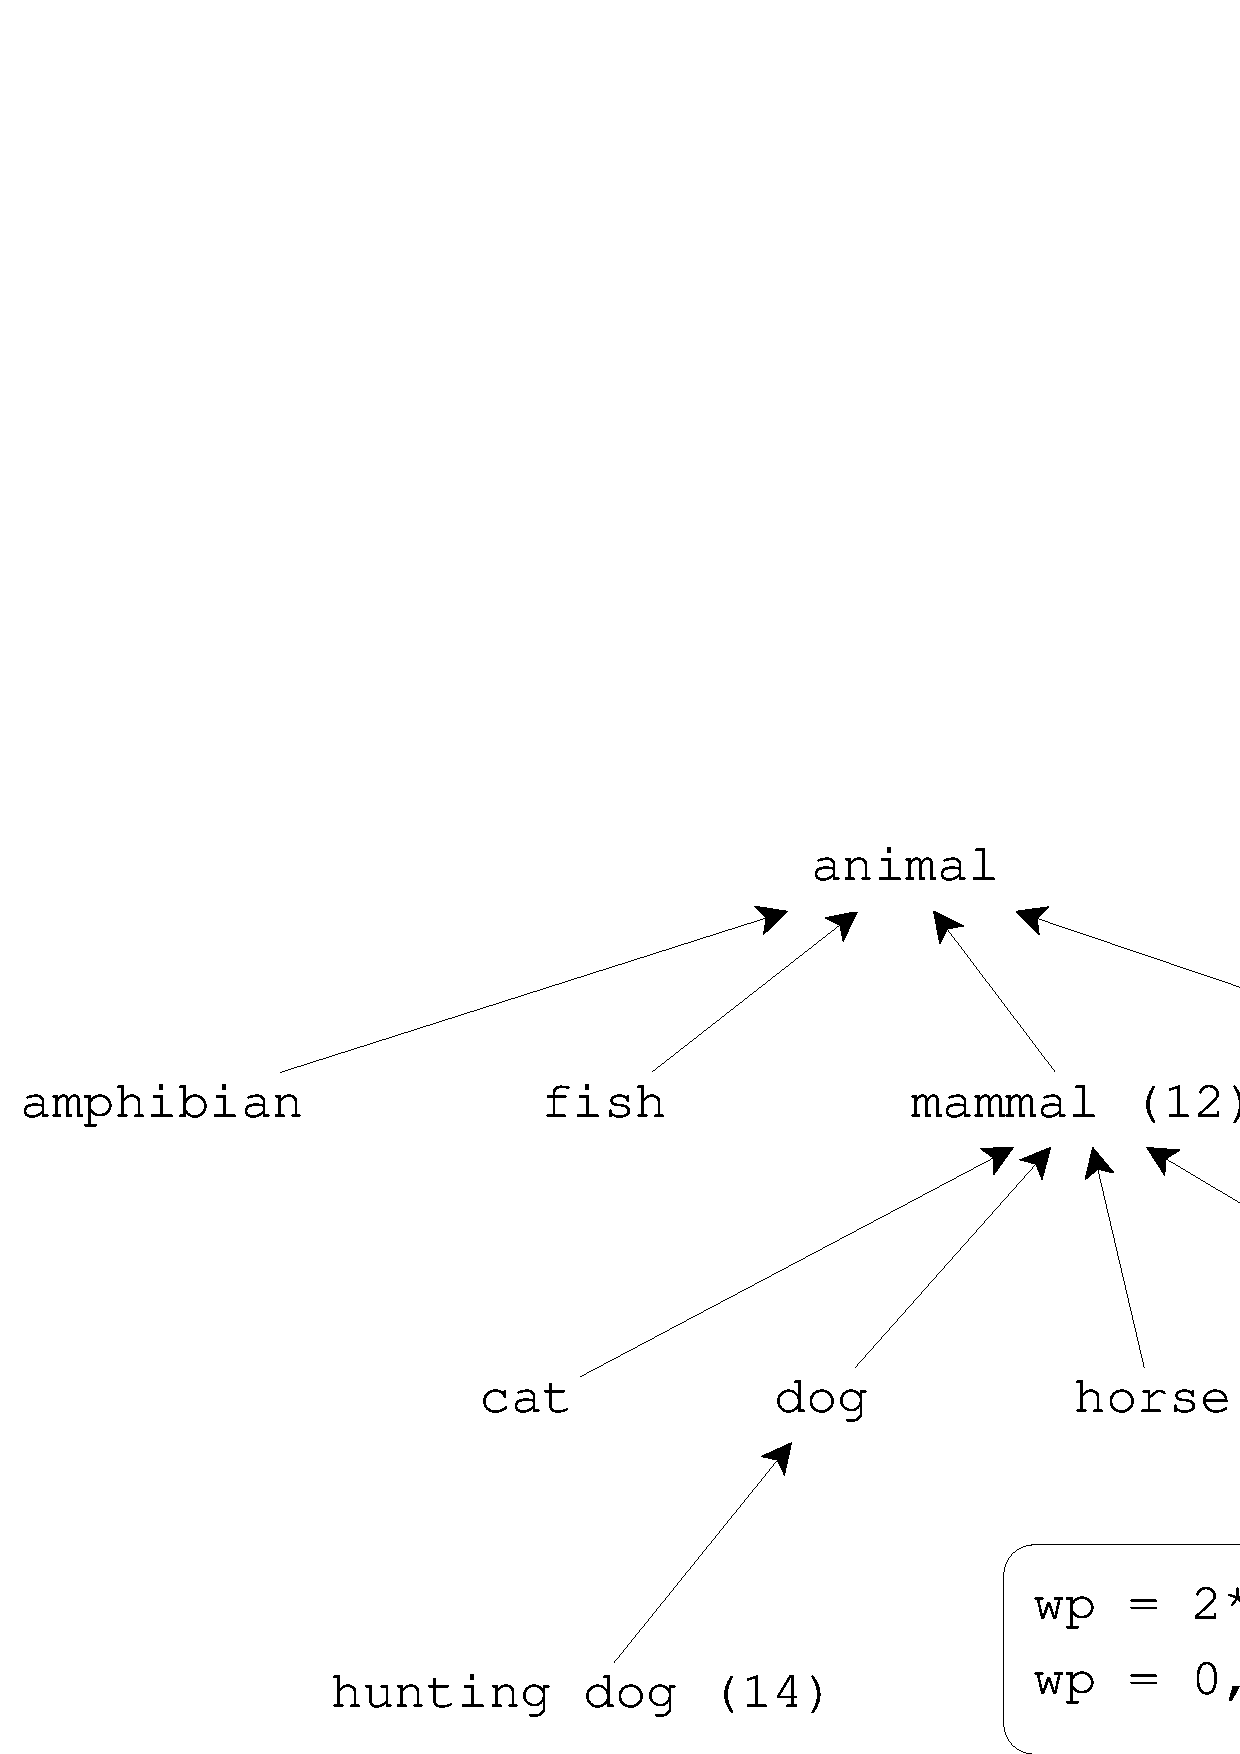
\includegraphics[width=\textwidth]{fig-002.png} %urna-2020.jpeg
			\caption{Urna Eletrônica utilizada no Brasil, a partir de 2022, do tipo DRE}
			\label{fig_urna_nova}
			\source{\textcite{urna-2020}.}
		\end{minipage}
	\end{figure}
	
	
	Quanto às gerações das UEs, \textcite{brunazo2016modelos} detalhou as três gerações de urnas eletrônicas utilizadas em eleições. 
	
	
	\begin{itemize}
		
		\item Primeira Geração - \textbf{\emph{Direct Recording Electronic - DRE}}: em português, Gravação Eletrônica Direta, surgiu nos anos 1990 e tinha como principal característica armazenar o voto apenas eletronicamente, sem possibilitar auditoria. Nestas urnas, a confiança no resultado era dependente apenas da confiabilidade no software instalado.
		\item Segunda Geração - \textbf{\emph{Voter Verifiable Paper Audit Trail - VVPAT} ou \emph{Independet Voter Verifiable Record - IVVR}}: surgiu no ano 2000 e ficou conhecida por permitir uma auditoria através de registros independentes do sistema, para cada voto, além do registro digital das máquinas DRE. Uma aplicação desse tipo de máquina é permitir que o usuário confira seu voto, através de uma cédula impressa pela máquina no ato do registro e deposite em uma outra urna.% Esta urna com as cédulas pode servir como estratégia de auditoria ao ter suas cédulas contadas e comparadas com o resultado disposto no boletim da urna. Com essa estratégia, estas urnas atingiram o princípio da independência do software \cite{rivest2008notion}, conceito que só fora formalizado depois e se tornou requisito em vários países.
		\item Terceira Geração - \textbf{\emph{End-to-End Verifiability - E2E Verifiability}}: Não é representada por um modelo específico de máquinas mas por inovações que tinham como característica aprimorar ou facilitar o processo de auditoria das eleições. Todos esses sistemas tinham em comum a independência do software e a auditoria independente de ponta a ponta no processamento do voto.% Por isso ficou conhecida como esse nome.
		
		%%\end{itemize}
	\end{itemize}
	
	
	No Brasil, a única geração de urna eletrônica até os dias atuais foram as urnas de primeira geração. Apesar disto, as urnas eletrônicas utilizadas nas eleições não foram do mesmo modelo. O TSE, que mantém e gerencia o processo de votação no Brasil, alterou a urna com o passar do tempo, inclusive para modernizá-la e trazer mais transparência aos processos de votação. Entretanto, pelo fato do método de registro de voto ser o DRE, considera-se que as UEs do Brasil são de primeira geração. Segundo \textcite{brunazo2016modelos}, os outros países que utilizam votação eletrônica nos seus processos de eleição, já abandonaram o uso das urnas de primeira geração, sendo o Brasil o único a ainda utilizá-la. %\textcite{ferrao2019urnas}, fez um mapeamento das alterações nas urnas feitas pelo TSE, além do processo de transição do voto de papel para o eletrônico. Este mapeamento pode ser conferido na \Cref{map-urnas}.
	
	
	% \begin{comment}
	% 	\begin{figure}[htbp]
	% 		\centering
	% 		\begin{minipage}{.8\textwidth}
	% 			\includegraphics[width=\textwidth]{mapeamentoFerrao.png}
	% 			\caption{Linha do tempo das urnas eletrônicas no Brasil}
	% 			\label{map-urnas}
	% 			\source{\textcite{ferrao2019urnas}.}
	% 		\end{minipage}
	% 	\end{figure}
	% \end{comment}
	
	
	%Segundo \textcite{brunazo2016modelos}, os outros países que utilizam votação eletrônica nos seus processos de eleição, já abandonaram o uso das urnas de primeira geração, sendo o Brasil o único a ainda utilizá-la.
	
	Foram encontradas brechas de segurança nas UEs, através dos Testes Publicos de Segurança, organizado pelo TSE, e apresentadas em \textcite{aranha2013vulnerabilidades,aranha2019return}. \textcite{aranha2019return} discutem ainda que a UE brasileira ainda não atende os requisitos mínimos de segurança e transparência e que não está desenvolvida o suficiente para uma aplicação de missão crítica de 20 anos. Sugere ainda a adoção de mais medidas de segurança, e a possível adoção de sistemas de \emph{software} independente, como as outras duas gerações de urna. Para ele, o maior desafio da adoção destas tecnologias é o entendimento do TSE de que anexar registros físicos ao sistema compromete o sigilo do voto. Apesar disto, após discursos de ataque a segurança da UE em 2021, \textcite{aranha-2021} reforçou não haver evidências de fraude no uso das UEs brasileiras e que sua defesa ao voto impresso (urnas de segunda geração) é apenas por mais transparência ao sistema eleitoral.
	%Estes trabalhos reproduzem os resultado obtidos através dos testes exploratórios da UE em período e ambiente controlado pelo TSE, pela equipe de testes. Em resumo, algumas vulnerabilidades encontradas nas urnas são as seguintes:
	
	% \begin{comment}
		
	% 	\begin{itemize}
	% 		\item Proteção inadequada do sigilo de voto, onde apesar dos votos serem armazenados fora de ordem no Registro Digital de Voto (RDV), é possível reverter o embaralhamento e descobrir a ordem verdadeira dos votos, quebrando seu sigilo;
	% 		\item Cifração inadequada: vulnerabilidade encontrada em ambos os testes e se refere ao fato de que a mesma chave criptográfica é utilizada para cifrar todas as urnas, o que possibilita o poder de todas as urnas a quem possuir a chave;
	% 		\item Uso de bibliotecas sem assinatura digital para autenticação ou algum outro tipo de verificação de integridade, o que permite a injeção de código arbitrário em suas funções;
	% 		\item Os testadores conseguiram injetar código para quebrar o sigilo do voto, manipulando chaves criptográficas em tempo real, utilizando um teclado normal e manipular registros de \emph{log} do sistema;
	% 		\item Os testadores foram capazes de injetar código para manipular \emph{strings} exibidas ao leitor em tempo real e anunciar um candidato hipotético.
	% 	\end{itemize}
		
	% \end{comment}
	
	
	
	
	\subsection{Votação Eletrônica (E-Voting)}
	
	E-voting é caracterizado por todo modelo que faça uso de qualquer meio de tecnologia, parcial ou totalmente, durante seu processo de votação \apud{kersting2004electronic, lacerda2019estudo} \cite{10061373, 9812616}. O modelo de votação eleitoral brasileiro atual, e de vários outros países, se encaixa neste modelo por utilizarem urnas eletrônicas e outros dispositivos. Fora do espectro eleitoral, são diversos os exemplos do uso do e-voting, como eleições informais, enquetes online, votação para programas de entretenimento, e eleições para cargos específicos.
	
	%Na história, uma aplicação inicial do uso do e-voting foi o uso de redes telefônicas para permitir o voto por conveniência. Por isso pessoas com deficiência podem votar em suas casas, e desde 1997, é permitido que os astronautas participem das eleições dos EUA \cite{gronke2008convenience} apud \cite{gibson2016review}. 
	
	Atualmente, o e-voting é prática mais recorrente devido ao avanço das tecnologias da informação. Em vários países, é comum associar o e-voting a UE, entretanto, existem outras abordagens de eleições com uso da tecnologia, inclusive de forma remota. Desde 2005, a Estônia permite a votação eleitoral de forma remota, através do aplicativo iVoting, a partir de qualquer dispositivo conectado à internet \cite{fornasier2022democracia}. Cerca de 46,7\% do estonianos utilizam o sistema para votar\footnote{Fonte: site oficial do projeto e-Estonia (https://e-estonia.com/solutions/e-governance/e-democracy/)}. Por depender de um ou mais canais de comunicação para realizar a eleição, estes sistemas apresentam desafios técnicos em relação à verificabilidade, confiabilidade, segurança, anonimato e confiança \cite{gibson2016review}.
	
	%Apesar de existir vários escopos da aplicação da votação eletrônica, um sistema de e-voting que visa ser seguro e efetivo deve seguir alguns princípios em seu projeto. Por isso, na \Cref{requisitos-eleicao}, são tratados alguns princípios de projeto de um sistema de votação eletrônica.
	
	
	
	\subsection{Requisitos para um Sistema de Votação Eletrônica Seguro}\label{requisitos-eleicao}
	
	\textcite{gritzalis2002principles} propôs alguns conceitos interessantes que foram usados como base para a definição de requisitos de outros trabalhos. Estes conceitos se complementam e se contradizem em algum ponto, sendo impossível projetar um sistema que atenda todos, entretanto, devem ainda ser considerados. Os princípios sugeridos por \textcite{gritzalis2002principles} são baseados na premissa de atender seis requisitos constitucionais. Estes requisitos são Generalidade, Liberdade, Igualdade, Sigilo, Eleição Direta e Democracia, e deram origem a 15 princípios. A seguir, estes requisitos são listados, assim como os princípios gerados por cada um dos requisitos. Para um maior aprofundamento sobre os requisitos e seus princípios, recomenda-se a leitura do trabalhos de \textcite{Soares_Vasconcelos_2023, gritzalis2002principles}.
	
	\begin{itemize}
		\item Generalidade;
		\begin{itemize}
			\item Isomorfismo ao Processo Tradicional;
			\item Elegibilidade ao Voto;
			\item Incoercibilidade;
			\item Não propaganda no sistema de votação;
			\item Capacidade de voto inválido.
		\end{itemize}
		\item Liberdade;
		\item Igualdade;
		\begin{itemize}
			\item Igualdade de Candidatos;
			\item Igualdade de Eleitores;
			\item Voto único.
		\end{itemize}
		\item Sigilo;
		\begin{itemize}
			\item Sigilo;
			\item Equilíbrio entre transparência e sigilo.
		\end{itemize}
		\item Eleição Direta;
		\begin{itemize}
			\item Voto não monitorado.
		\end{itemize}
		\item Democracia.
		\begin{itemize}
			\item Confiança e transparência;
			\item Verificabilidade e prestação de contas;
			\item Confiabilidade e segurança;
			\item Simplicidade.
		\end{itemize}
	\end{itemize}
	
	
	% \begin{comment}
	% 	\subsubsection{Generalidade \label{principio-generalidade}}
		
	% 	Este requisito constitucional relembra que os sistemas de votação devem ser acessíveis para todos, independentemente de alfabetização, classe, renda, etnia ou sexo, ou seja, deve ser baseado na ideia de sufrágio universal. A fim de atingir este requisito, surgem dois princípios:
		
	% 	\textbf{Princípio do Isomorfismo ao Processo Tradicional}
		
	% 	Este princípio remete principalmente à obrigação do sistema possuir a característica de sufrágio universal, dos meios tradicionais. Assim, este princípio está dividido em cinco tópicos, que são eles:
		
		
	% 	\begin{itemize}
	% 		\item Todo eleitor tem direito de participar do processo eleitoral;
	% 		\item A elegibilidade para participar do processo de votação deve ser fundamentado e regulamentado por lei (para eleições nacionais);
	% 		\item A tecnologia de votação deve ser acessível para todos;
	% 		\item A votação eletrônica deve ser considerada uma forma alternativa para o direito de voto;
	% 		\item O princípio democrático, ou seja, que todos tem direito a participar do processo de votação, exige uma infraestrutura pública apropriada disponível para uso dos cidadãos.
	% 	\end{itemize}
		
	% 	\textbf{Princípio da Elegibilidade ao Voto}
		
	% 	Este princípio propõe que a elegibilidade possa ser assegurada através do registro e autenticação de eleitores elegíveis. Estes procedimentos visam garantir o sufrágio universal, uma vez que permite que apenas votantes aptos possam votar e só faça isso uma vez.
		
	% 	\textbf{Liberdade}
		
	% 	Este requisito se baseia na premissa que um eleitor deve possuir total liberdade para escolher e votar em um candidato durante a eleição, não devendo sofrer influência, pressão ou manipulação pelo estado ou outros indivíduos. A fim de garantir esta liberdade, surgem três princípios.
		
	% 	\textbf{Princípio da Incoercibilidade} \label{icoercibilidade}
		
	% 	Este princípio visa garantir que o eleitor não venda seu voto ou seja cobrado pelo mesmo. Com esse objetivo, é necessário que não exista associação entre o votante e seu voto, seja através de comprovantes ou no próprio sistema. Deve-se garantir também que o eleitor não seja coagido fora do sistema, através de uma estrutura de votação adequada.
		
	% 	\textbf{Princípio da não propaganda no sistema de votação}
		
	% 	Este princípio visa garantir que o sistema forneça liberdade para que o eleitor escolha seu voto. Para isso, o sistema deve ser imparcial e isento de qualquer propaganda ou referência a candidatos aos cargos em eleição.
		
	% 	\textbf{Princípio da capacidade de voto inválido} \label{capacidade-voto-invalido}
		
	% 	Este princípio visa permitir que o eleitor ainda participe do processo de votação ainda que acredite que nenhum candidato lhe representa. Para isso, o sistema deve computar votos nulos ou em branco.
		
	% 	\subsubsection{Igualdade}
		
	% 	Este requisito é baseado no conceito propriamente dito de igualdade, e se aplica a eleitores e candidatos. A partir deste princípio surgem três princípios.
		
	% 	\textbf{Princípio da Igualdade de Candidatos}
		
	% 	Este princípio visa garantir a igualdade dos candidatos de modo que nenhum candidato seja privilegiado ou prejudicado pelo sistema, isto é, votos com peso maior, votos duplicados, votos não computados e etc. O sistema deve garantir que todos os candidatos sejam expostos as mesmas condições.
		
	% 	\textbf{Princípio da Igualdade de Eleitores}
		
	% 	Este princípio visa garantir a igualdade dos eleitores perante o sistema. Nenhum eleitor ou grupo de eleitores deve possuir vantagem ou desvantagem durante o ato do voto. Situações que eleitores possuem maior peso de voto, ou que não conseguem votar em algum candidato não devem acontecer. No ponto de vista do sistema, os eleitores devem ser iguais. Ainda, fora do sistema, os eleitores devem possuir igualdade também, principalmente no que diz respeito ao acesso. O sistema deve ser acessível para todos os eleitores, de maneira igualitária.
		
	% 	\textbf{Princípio do voto único}
		
	% 	Este princípio está associado ao último princípio, e é baseado na premissa que cada eleitor só pode votar uma vez. Ou seja, o voto de cada eleitor deve ser computado com o mesmo peso e valor, reforçando a igualdade entre os eleitores.
		
	% 	\subsubsection{Sigilo}
		
	% 	Este requisito está relacionado com o requisito de Liberdade e tem o principal objetivo de garantir o sigilo da escolha individual de cada eleitor. Este requisito pode ser considerado como um princípio propriamente dito, como será disposto na seção seguinte.
		
	% 	\textbf{Princípio de sigilo}
		
	% 	Este princípio visa principalmente garantir a liberdade de escolha do indivíduo e coibir a coercibilidade e possíveis consequências ao eleitor após o registo do seu voto. Para isto, este princípio é dividido em quatro pontos-chave:
		
	% 	\begin{itemize}
	% 		\item O sigilo do voto deve ser garantido durante todo o processo (emissão do voto, registro, transmissão e apuração);
	% 		\item Nenhum dos atores envolvidos no processo de votação (Organizadores, funcionários, eleitores e etc) deve ser capaz de associar um eleitor a um voto;
	% 		\item Deve existir no sistema uma separação entre os processos de autenticação e os de registro de voto;
	% 		\item O eleitor não deve ser capaz de provar em quem votou.
	% 	\end{itemize}
		
	% 	Este último item pode ser atingido através da não emissão de comprovantes de votação pelo sistema.
		
	% 	\textbf{Princípio do equilíbrio entre transparência e sigilo}
		
	% 	Apesar da necessidade dos sistema garantir o sigilo, também é imprescindível que o sistema seja transparente, para que esteja de acordo com outros princípios democráticos. Por isso, é necessário haver um equilíbrio entre estes pontos, garantindo que o sistema seja auditável, permitindo autenticidade de boletim de votos e permitindo recontagem, sem identificar eleitores.
		
	% 	\subsubsection{Eleição Direta}
		
	% 	Este requisito requer que não possua intermediários no processo de decisão do voto. Um desses intermediários poderia ser a contagem em tempo real dos votos, principalmente caso exista mais de uma alternativa de votação. Resultados de votações \emph{online} poderiam interferir nos resultados das votações \emph{offline}. Por isso, para suprir esta necessidade, surge o requisito disposto na seção seguinte.
		
	% 	\textbf{Princípio do voto não monitorado}
		
	% 	Este princípio visa impedir que os votos possam sofrer interferência durante o processo. Uma solução é impedir que a urna seja aberta antes do encerramento do processo de votação. O mesmo se aplica aos sistema de votação eletrônica, que deve apenas disponibilizar o resultado da contagem após o encerramento da sessão de votos. A quebra deste princípio permite a monitoração de votos pela entidade que armazena os votos e ainda pode permitir associar um eleitor a um voto, quebrando o princípio de sigilo.
		
	% 	\subsubsection{Democracia}
		
	% 	Este talvez seja o requisito mais importante para a validade de um sistema de votação. Para um sistema de votação eletrônica, faz-se necessário que atinja pelo menos os mesmos requisitos de um sistema tradicional de votos. A partir deste requisito surgem quatro princípios importantes.
		
	% 	\textbf{Princípio da confiança e transparência}
		
	% 	Um sistema de votação deve ser transparente e confiável para os eleitores e outros atores. Nos sistemas eletrônicos, indivíduos que não conhecem o sistema de maneira técnica devem confiar no processo, por isso o sistema deve ser transparente e as autoridades responsáveis devem informar o meio que as eleições são conduzidas a fim de atingir a confiabilidade no sistema.
		
	% 	\textbf{Princípio da verificabilidade e prestação de contas}
		
	% 	Este princípio remete a capacidade do eleitor e outros atores verificarem se o sistema está funcionando como se espera. Para isso, o eleitor deveria ser capaz de ter certeza que seu voto foi computado e as instituições, de prestar contas, através de \emph{logs} de monitoramento. Entretanto, este princípio entra em conflito com o princípio de sigilo, por isso, o princípio de equilíbrio entre sigilo e transparência deve ser consultado. Segundo \textcite{Soares_Vasconcelos_2023}, de modo geral, este princípio é abdicado em favor da manutenção do sigilo.
		
	% 	\textbf{Princípio da confiabilidade e segurança}
		
	% 	Este princípio remete a confiabilidade que o sistema reproduzirá um resultado correspondente aos votos expressos, sem sofrer interferência ou manipulação. Todos os votos devem ser computados, inclusive os brancos e nulos, e nenhum voto deve ser perdido. Em outras palavras, o sistema deve ser íntegro. 
	% 	Quanto a segurança, o sistema deve possuir garantias técnicas a respeito da disponibilidade, sigilo, integridade, registro, elegibilidade e autenticação. Além disso, o sistema deve ser proibido de ter intervenções externas, acidentais ou não, que causem indisponibilidade do sistema. O sistema ficar indisponível pode impactar no direito de voto dos cidadãos.
		
		
	% 	\textbf{Princípio da simplicidade}
		
	% 	Este princípio está associado com acessibilidade e parte da necessidade da simplicidade do sistema para que funcione corretamente e possa ser utilizado de maneira satisfatória e sem complicações. Obviamente, garantir os princípios anteriores podem exigir de certa complexidade do sistema, mas isto pode ser resolvido com treinamento, reengenharia, suporte e etc, que permitem uma abstração da complexidade e provem uma acessibilidade por meio dos eleitores.
		
	% 	Com isso, \textcite{gritzalis2002principles} propõe sete requisitos para sistema de votação eletrônica:
		
	% 	\begin{itemize}
	% 		\item Devem existir processos de certificação dos \emph{hardwares} e \emph{softwares} envolvidos no sistema;
	% 		\item Toda infraestrutura e funcionalidades devem ser verificáveis;
	% 		\item Todos os eventos realizados no sistema devem ser monitorados, desde que permaneça o sigilo individual dos eleitores;
	% 		\item A infraestrutura deve ser aberta para inspeção de agentes autorizados;
	% 		\item Os atores envolvidos na eleição devem ter certeza que não houve má prática;
	% 		\item O sistema deve garantir segurança adequada;
	% 		\item O sistema deve ser acessível e fácil de usar.
	% 	\end{itemize}
		
	% \end{comment}
	
	\subsection{\emph{Blockchain}}
	
	\emph{Blockchain} é uma estrutura de dados onde só é permitida a adição de dados, assim, os dados são inseridos em blocos de modo que cada bloco possui o \emph{hash} do bloco anterior \cite{nakamoto2008bitcoin}. Além disso, as redes \emph{blockchain} funcionam sob o controle de um livro-razão, isto é, a cada vez que uma transação ocorre, o algoritmo do contrato inteligente é executado e o resultado é registrado no livro-razão de todos os nós. \emph{Blockchain} é uma forma de tecnologia de contabilidade distribuída na qual as transações são registradas através de valores \emph{hashes}, que são valores fixos gerados através de um algoritmo \emph{hash} para um código de valor variável. Se este valor for alterado e submetido ao mesmo algoritmo, o resultado será totalmente diferente. Isso pressupõe que, se um único bloco em uma cadeia for modificado, fica claro que a cadeia foi adulterada, e isso torna difícil alterar, \emph{hackear} ou enganar o sistema. A partir dessa lógica, é possível aplicar tais conceitos para diversos contextos \apud{mingxiao2017review, cadiz2021empirical} \cite{10061373}. Nesse contexto, as diversas redes \textit{blockchain} podem ser classificada em públicas ou privadas (também conhecidas como permissionadas).
	%Esta rede foi criada por \textcite{nakamoto2008bitcoin} para suprir as necessidades de sua aplicação de criptomoedas, o \emph{Bitcoin}.
	
	% \begin{comment}
	% 	\begin{figure}[htbp]
	% 		\centering
	% 		\begin{minipage}{.8\textwidth}
	% 			\includegraphics[width=\textwidth]{blocos-nakamoto.png}
	% 			\caption{Encadeamento de blocos de redes \textit{blockchain}}
	% 			\label{encadeamento}
	% 			\source{\textcite{nakamoto2008bitcoin}.}
	% 		\end{minipage}
	% 	\end{figure}
	% \end{comment}
	
	%Além disso, as redes \emph{blockchain} funcionam sob o controle de um livro-razão, isto é, a cada vez que uma transação ocorre, o algoritmo do contrato inteligente é executado e o resultado é registrado no livro-razão de todos os nós. \emph{Blockchain} é uma forma de tecnologia de contabilidade distribuída na qual as transações são registradas através de valores \emph{hashes}, que são valores fixos gerados através de um algoritmo \emph{hash} para um código de valor variável. Se este valor for alterado e submetido ao mesmo algoritmo, o resultado será totalmente diferente. Isso pressupõe que, se um único bloco em uma cadeia for modificado, fica claro que a cadeia foi adulterada, e isso torna difícil alterar, \emph{hackear} ou enganar o sistema. A partir dessa lógica, é possível aplicar tais conceitos para diversos contextos \cite{mingxiao2017review} apud \cite{cadiz2021empirical}.
	
	%Nesse contexto, as diversas redes \textit{blockchain} podem ser classificada dentre alguns fatores. Uma classificação bem comum é acerca do nível de proteção de dados. Algumas redes, chamadas de públicas ou não permissionadas, como a \textit{Bitcoin} e \textit{Ethereum}, vários computadores anônimos podem cooperar entre si para armazenar e semear informações com segurança, de modo que os nós podem entrar ou sair da rede a qualquer momento. Redes desse tipo são mais lentas e menos privados que bancos de dados tradicionais. Já as redes permissionadas, adicionam uma camada de autenticação na rede, reduzindo o problema de confiança entre os membro mas sem ônus de funcionalidades em relação as públicas \cite{peck2017blockchain}.
	% \hl{ }
	% \begin{comment}
	% Em resumo, segundo \textcite{dannen2017introducing}, \textit{blockchain} é a combinação de três tecnologias:
	% \begin{itemize}
	% 	\item Rede Ponto a Ponto: grupo de computadores que podem se comunicar entre si sem depender de uma única autoridade central.
	% 	\item Criptografia Assimétrica: uma maneira que esses computadores podem enviar mensagens criptografadas para destinatários específicos, de modo que qualquer pessoa pode verificar a autenticidade da mensagem mas não o conteúdo.% Nas redes \textit{Bitcoin} e \textit{Ethereum} essa tecnologia é utilizada para criar credenciais para que apenas o dono da conta possa transferir seus \textit{Tokens}.
	% 	\item \textit{Hash} criptográfico: Uma maneira de gerar uma "\textit{impressão digital}" para qualquer dado, que permite comparar grandes volumes de dados e ter certeza que eles não foram alterados.% Nas redes \textit{Bitcoin} e \textit{Ethereum}, a estrutura de dados ''\textit{Árvore de Merkle}''\footnote{\textit{Merkle Tree} - \textcite{merkle1980protocols}} (\Cref{markle-tree}) é utilizada para garantir a ordem das transações, sendo criptografada em forma de \textit{hash} e serve de comparação entre os computadores.
	% \end{itemize}
	% \end{comment}
	
	% \begin{comment}
	% 	\begin{figure}[htbp]
	% 		\centering
	% 		\begin{minipage}{.8\textwidth}
	% 			\includegraphics[width=\textwidth]{Merkle tree.png}
	% 			\caption{Árvore de Merkle}
	% 			\label{markle-tree}
	% 			\source{\textcite{enwiki:1159724280}.}
	% 		\end{minipage}
	% 	\end{figure}
	% \end{comment}
	
	Neste tipo de rede, surge ainda o conceito de \emph{Smart Contracts}, ou Contratos Inteligentes, que são contratos programáveis executados automaticamente quando certas condições pré-definidas são atendidas. Estes contratos automatizam as transações e permitem que as partes cheguem a acordos sem a necessidade de uma entidade intermediária. Além disso, estes contratos são acessíveis por todos os usuário da rede, o que permite sua auditoria \cite{hjalmarsson2018blockchain, Tanwar2024}.
	
	
	\subsection{\emph{Blockchain} e E-Voting}
	
	Pelos benefícios que o conceito de \emph{blockchain} traz, principalmente de imutabilidade de dados registados, contratos inteligentes públicos e possibilidade de acesso por todos os nós da redes, é possível aplicar este conceito em \textit{e-voting}. Vários são os benefícios do uso de \emph{blockchain} para votação. Uma vez que a integridade do sistema eleitoral é fundamental para integridade da própria democracia \cite{kohno2004analysis}, o uso de tecnologias de \emph{blockchain} são convenientes para um sistema de votação por possibilitar maior transparência e auditabilidade, maior eficiência, menor susceptibilidade a erros e falhas humanas, e redução de custos %\hl{ }
\cite{fornasier2022democracia, 10.1007/978-981-19-1976-3_18, Tanwar2024, electronics13010017}.
	
	%Por isso, recentemente é cada vez mais comum a utilização dessas redes em diversas aplicações. A mais comum delas são as relacionadas à valores financeiros, como as criptomoedas, entretanto, existem outras possíveis aplicações interessantes. %A \emph{Walmart}, diante de problemas de consenso em pagamentos de suas 70 distribuidoras no Canadá, começou a testar o uso de redes \emph{blockchain} em  2019 para unificar sua base de dados para todas as distribuidoras, com os dados acessíveis à todas elas. Com esses dados acessíveis e unificados, a discrepância entre as faturas do \emph{Walmart} e das distribuidoras caiu significativamente. Antes do uso da rede \emph{blockchain}, cerca de 70\% das faturas eram contestadas, e depois, apenas 1\% \cite{vitasek2022walmart}.
	
	%Entretanto, essas aplicações não se restringem à iniciativa privada. Dubai possui desde 2020 a iniciativa de integrar todos seus sistemas públicos a redes de \emph{blockchain}, visando modernidade e redução de custos, através do projeto \emph{Dubai blockchain Strategy\footnote{https://www.digitaldubai.ae/initiatives/\emph{blockchain}}}. Voltando para o Brasil, já é de iniciativa da Receita Federal do Brasil o uso de \emph{blockchain} para disponibilização de dados como CPF e CNPJ, através dos projetos b-CPF e b-CNPJ, onde o ''b'' se refere a \emph{blockchain} \cite{thompson2019projeto}.
	
	%Especificamente sobre votação, já existem aplicações de votação que fazem o uso de redes \emph{blockchain} para armazenamento seguro dos votos. \textcite{sepulvida2019estudo} destacam em seu trabalho uma dessas plataformas, chamada de \emph{FollowMyVote\footnote{https://followmyvote.com/}}. Esta plataforma de código aberto, isto é, com código fonte auditável, possibilita o processo de votação remoto através da instalação da aplicação em um dispositivo com validação digital através de foto, e registro do voto. Além disso, o votante pode ver a contagem de votos em tempo real.
	
	%Vários são os benefícios do uso de \emph{blockchain} para votação. Uma vez que a integridade do sistema eleitoral é fundamental para integridade da própria democracia \cite{kohno2004analysis}, o uso de tecnologias de \emph{blockchain} são convenientes para um sistema de votação por possibilitar maior transparência e auditabilidade, maior eficiência, menor susceptibilidade a erros e falhas humanas, e redução de custos \cite{fornasier2022democracia}.
	
	Com a remodelagem do sistema, algumas brechas de segurança da UE atual podem ser resolvidas, como o possível desembaralhamento do RDV. Com os votos salvos em uma base única, é mais difícil identificar os votantes a seus respectivos votos. Além disso, outra vantagem seria a confiabilidade no sistema. É claro que a integridade da eleição ainda dependeria da boa-vontade daqueles que o desenvolvem, mas com os contratos inteligentes públicos, ou com iniciativas \emph{opensource}, o sistema pode ser auditado e verificado acerca do seu funcionamento.
	
	O uso de \emph{blockchain} associado a ''sistemas eletrônicos para votação estão sendo desenvolvido e aperfeiçoado em diversos lugares do mundo, com a proposta de gerar mais confiabilidade e clareza aos eleitores'' \cite{sepulvida2019estudo}. Entretanto, um projeto de \emph{E-voting}, para eleições de grande porte, como a eleição federal brasileira onde são computador centeas de milhões de votos, é necessário garantir o funcionamento e a viabilidade da estrutura. 
	
	Ademais, aplicar um novo modelo descentralizado de votação vai além da possibilidade técnica. ''A implementação de sistemas de votação eletrônica com a tecnologia \emph{blockchain} ainda encontra dificuldades (jurídicas), especialmente aquelas diretamente relacionadas às políticas vigentes em cada país'' \cite{sepulvida2019estudo}.  Segundo \textcite{gibson2016review}, alterar a forma como as pessoas votam tem muitas implicações sociais e políticas, principalmente porque o papel dos administradores eleitorais são completamente diferentes quando estas tecnologias estão envolvidas. Segundo \textcite{silvapassos2018}, existe a possibilidade tanto técnica quanto jurídica de realizar a implantação da tecnologia \emph{blockchain} no sistema eletrônico de votação brasileiro. Ele menciona ainda que esta tecnologia é relativamente nova e que deve ser testada para comprovar real eficácia, mas que isso não deve se tornar um empecilho à sua utilização. 
	
	\subsection{\textit{Ethereum, Solidity} e o \textit{Projeto Remix}}
	
	O \textit{Ethereum} é uma rede \textit{blockchain open source}, que assim como o \textit{Bitcoin}, permite a criação de um sistema econômico completo, com gerenciamento de contas e uma moeda nativa.  Nesta rede, é possível criar e publicar contratos inteligentes, os quais são a lógica de negócio que é executada na rede, fazendo-se cumprir acordos de pagamento entre as partes.% Estes contratos se parecem com o conceito de classes na programação orientada a objetos convencional \cite{dannen2017introducing}. 
	
	Uma das linguagens mais utilizadas para escrever os contratos é \textit{Solidity}\footnote{Solidity: https://soliditylang.org/}. Ela uma linguagem de alto nível orientada a contratos com traços da linguagem C e JavaScript. Assim como o \textit{Ethereum}, \textit{Solidity} também é uma tecnologia de código aberto.% Os contratos são publicados de maneira gratuita, entretanto, existe um custo das transações \cite{dannen2017introducing}.
	
	Um conceito importante sobre as redes \textit{Ethereum} e as \textit{EVM} (\textit{Ethereum Virtual Machine}) é o conceito de \textit{Gas}. Embora publicar contratos na rede seja grátis, as transações são mantidas mediante um custo associado e cada vez que um usuário realiza uma transação, um valor é pre-reservado de sua carteira para arcar com esses custos. O \textit{Gas} é a unidade de medida usada para mensurar esse custo, representando uma pequena fração de um \textit{Ether}. Além de manter os custos,  o \textit{Gas} serve para uma outra finalidade que é garantir que os programas executados sejam finalizados, uma vez que possuem um limite de custo, que quando atingido, encerra a transação \cite{dannen2017introducing}. 
	
	Por fim, existe o \textit{Remix Project}\footnote{\emph{Remix Project}: https://remix-project.org/}, que é uma ferramenta de desenvolvimento de contratos da rede \textit{Ethereum}. Por meio desta ferramenta é possível, escrever, compilar, publicar e testar contratos, tanto em rede local ou na rede \textit{Ethereum}. Após a criação, é possível usar uma conta real para se conectar ao contrato, mas para isso precisa ter saldo de \textit{Ether} (moeda nativa da rede) para efetuar a transação. 
	
	% \begin{comment}
		
	% 	\begin{figure}[htbp]
	% 		\centering
	% 		\begin{minipage}{1\textwidth}
	% 			\includegraphics[width=\textwidth]{Remix.jpg}
	% 			\caption{\textit{Dashboard} da plataforma Remix.}
	% 			\label{fig:remix}
	% 			\source{Autor.}
	% 		\end{minipage}
	% 	\end{figure}
		
	% 	A \Cref{fig:remix} mostra a tela da aplicação web do projeto \textit{Remix}. A partir dela é possível acompanhar algumas funções através das marcações:
		
	% 	\begin{enumerate}
	% 		\item Região para fazer \textit{deploy} dos contratos, podendo selecionar região, endereço, conta, limite de custos e etc.
	% 		\item Região para acompanhar os contratos publicados, suas transações possíveis e opções para execução.
	% 		\item Editor de texto do ambiente, onde pode-se escrever os contratos.
	% 		\item Região para acompanhar os resultados das transações, possíveis mensagens de erro, consumo e mais.
	% 	\end{enumerate}
		
	% \end{comment}
	
	\section{Proposta de E-voting Baseada em Blockchain \label{desenvolvimento}}
	
	Nesta seção é proposto um modelo de votação eletrônica descentralizado que terá como objetivo contribuir com mais transparência e segurança ao modelo atual através do uso de redes \emph{blockchain}, e a demonstração de um contrato inteligente desenvolvido.
	
	\subsection{Proposta do Sistema}
	
	Este modelo foi pensado para atuar em conjunto com o sistema atual de votação no registro, armazenamento e acesso dos votos. Nesta proposta, o eleitor ainda teria que registrar seu voto através de urna eletrônica, mas a consulta ao código do algoritmo de consenso e aos votos (após o período de eleições), será público. Cada UE funcionará como um nó de submissão de votos. Apenas nós deste tipo podem submeter votos, e por isso, os endereços de rede desses nós são previamente armazenados na rede. Qualquer outro dispositivo que se conecte à rede poderá consultar seus próprios dados (poderá ver comprovante de votação e dados pessoais), consultar os dados dos candidatos, e após a eleição, verificar a quantidade de votos que cada candidato recebeu. Quanto ao período de eleição, este deve ser cadastrado previamente e ser disposto no \emph{smart contract}, para que seja respeitado o tempo da sessão de votação e o momento em que as consultas de votos serão liberadas. 
	
	Dessa forma, uma definição formal da estrutura proposta é: uma composição de nós interligados baseados no conceito de \emph{blockchain}, possuindo um contrato inteligente definido com o propósito de garantir as regras de uma votação eletrônica segura, que permite o voto único por eleitor, a submissão de votos apenas por nós do tipo UE previamente registrados, e a divulgação automática dos resultados após o fim da eleição para qualquer nó conectado.
	
	\subsection{Estruturas e Atores do Sistema}
	
	
	Atualmente, o sistema eleitoral brasileiro é mantido pelo Tribunal Superior Eleitoral (TSE), com o apoio dos Tribunais Regionais Eleitorais (TREs), ambos responsáveis por administrar todo o processo eleitoral, desde o desenvolvimento e manutenção das UE, registro prévio de eleitores e candidatos, e eleição e apuração dos votos. No modelo proposto, uma Autoridade Eleitoral, semelhante ao que o TSE representa hoje, ainda terá responsabilidade, entretanto, outros atores participarão do processo, conforme \Cref{tab-relacao-autoridade}. Este modelo visa que com o uso da rede descentralizada, outros atores, além de uma Autoridade Eleitoral, possam acompanhar o processo. Quanto à estrutura, a comparação pode ser vista na \Cref{tab-relacao-componentes}.
	
	
	
	\begin{table}[htbp]
		\centering
		\caption{Comparação da relação de autoridade entre o modelo atual e o modelo proposto.}
		\label{tab-relacao-autoridade}
		\begin{tabular}{lll}
			\toprule
			\textbf{Responsabilidade} & \textbf{Modelo Atual} & \textbf{Modelo Proposto} \\
			\midrule
			Registrar Eleitores & Autoridade Eleitoral & Autoridade Eleitoral \\
			\midrule
			Registrar Candidatos & Autoridade Eleitoral & Autoridade Eleitoral \\
			\midrule
			Prover Estrutura & Autoridade Eleitoral & Autoridade Eleitoral \\
			\midrule
			Votar & Eleitores & Eleitores \\
			\midrule
			Registrar Votos & Autoridade Eleitoral & Blocos de registro da rede descentralizada \\
			\midrule
			Armazenar Votos & Autoridade Eleitoral & Qualquer bloco da rede descentralizada\\
			\midrule
			Apuração dos Votos & Autoridade Eleitoral & Eleitores, Candidatos, Autoridade, Cidadãos \\
			\bottomrule
		\end{tabular}
		\source{Autor.}
	\end{table}
	
	
	
	
	
	%É possível acompanhar da \Cref{tab-relacao-autoridade} que este modelo visa que com o uso da rede descentralizada, outros atores, além de uma Autoridade Eleitoral, possam acompanhar o processo.
	%Quanto à estrutura, a comparação pode ser acompanhada na \Cref{tab-relacao-componentes}.
	
	\begin{table}[htbp]
		\centering
		\caption{Comparação da estrutura do modelo atual e do modelo proposto.}
		\label{tab-relacao-componentes}
		\newcolumntype{Y}{>{\raggedright\arraybackslash}X}
		\begin{tabularx}{\textwidth}{YYY}
			\toprule
			\textbf{Componente} & \textbf{Modelo Atual}  & \textbf{Modelo Proposto} \\
			\midrule
			Dispositivo de Registro de Votos & UE de modelo DRE. & UE conectada a rede descentralizada. \\
			\midrule
			Modelo de Rede & Durante as sessões de votação, a UE não é conectada a alguma rede. & Rede \emph{blockchain} descentralizada com regras de registro e consulta. \\
			\midrule
			Modo de contagem de Votos & Contagem através da leitura dos cartões de memória das máquinas. & Consulta através de qualquer nó, após fim do período de votação. \\
			\bottomrule
		\end{tabularx}
		\source{Autor.}
	\end{table}
	
	O Ator \textbf{''Autoridade Eleitoral''} é a entidade responsável por gerir o pleito eleitoral. No Brasil é o TSE, e neste novo modelo a entidade terá o papel de produzir e projetar as novas UEs, desenvolver uma interface compatível e escrever um contrato inteligente para utilizar de maneira embarcada. Além disso, será preciso validar o registro dos candidatos e eleitores, que devem ser controlados para garantir a elegibilidade dos candidatos e prevenir a falsidade ideológica de eleitores. Deve também gerir todo o processo de votação no dia da eleição (disposição das urnas em zonas eleitorais, fiscalização do processo, etc.).
	
	O Ator \textbf{''Eleitor''} é o cidadão em plena execução dos seus direitos previamente identificado. Autentica-se durante o processo de votação e recebe confirmação que votou, embora não possa gerar nenhum comprovante de qual candidato escolheu.
	
	O Ator \textbf{''Candidato''} é o cidadão em plenas condições de exercer o cargo ao qual concorre e que está apto a receber votos.
	
	A \textbf{''Rede distribuída''} pode ser considerada um ator uma vez que possui grande importância no processo, é responsável por autenticar os eleitores durante o processo de votação, armazenar os votos, controlar as fases da votação e disponibilizar o resultado.% Este é um conceito abstrato, uma vez que a rede será uma composição de nós interligados.
	
	
	
	\subsubsection{Regras da Eleição e Fases}
	
	O modelo foi projetado levando com o objetivo de atingir da melhor maneira os princípios definidos na \Cref{requisitos-eleicao}. A partir disso, foram definidas regras e premissas foram definidas. 
	
	\textbf{Quanto à rede: }
	\begin{itemize}
		\item O modelo de comunicação é o de redes \emph{bockchain};
		\item O modelo é composto por nós descentralizados que se comunicam entre si;
		\item Os nós executarão um \emph{smart contract} com as regras de negócio da aplicação;
		\item Deve existir criptografia de dados durante a comunicação entre os nós, a fim de evitar interceptações;
		\item A rede deve ser não pressionada, para permitir a execução de transações por terceiros, facilitando a transparência durante a consulta;
		\item Qualquer nó conectado a rede poderá consultar votos e o contrato inteligente;
		\item Nós poderão executar papéis diferentes.
	\end{itemize}
	\textbf{Quanto às regras de negócio: }
	\begin{itemize}
		\item Cada eleitor pode registrar voto apenas uma vez;
		\item Nós do tipo Urna Eletrônica serão os únicos que podem registrar votos na rede. Seus endereços devem ser armazenados e pré-cadastrados antes da eleição.
		\item Qualquer outro nó não identificado como uma UE poderá consultar informações próprias (se for um eleitor), informações dos candidatos e consultar a contagem de votos ao final da eleição.
		\item O eleitor vota em um candidato através de um número de identificação único, semelhante ao que ocorre atualmente no sistema eleitoral brasileiro;
		\item Um eleitor pode verificar seu comprovante de votação, mas não pode obter qualquer comprovante de quem votou;
		\item Dados biométricos dos eleitores devem ser armazenados na rede para realizar autenticação;
		\item Votos nulos e brancos devem ser registrados;
		\item O contrato deve atender as restrições referentes as Fases da eleição;
		\item Nenhum voto é perdido ou adulterado, e caso isso acontecesse, seria possível a identificação através dos livro-razão dos blocos.
	\end{itemize}
	\textbf{Quanto às fases da eleição: }
	\begin{itemize}
		\item A eleição é dividida em três fases \cite{Soares_Vasconcelos_2023}.
		%Esta modelo utiliza uma definição semelhante à proposta por \textcite{Soares_Vasconcelos_2023} que divide o processo da eleição em três fases.
		\item Fase 1 - \emph{Setup} da eleição: Primeira parte do processo, cuja autoridade central deve construir a rede, validar candidaturas, registrar os eleitores aptos na rede e montar o esquema de eleição.
		\item Fase 2 - Registro de Votos: Período em que as seções permanecem abertas e o sistema está apto a receber votos dos blocos autorizados. 
		\item Fase 3 - Inicia-se após o encerramento da Fase 2 e corresponde ao período pós sessão de votação. Nesta fase,  os votos são divulgados.
		\item Candidatos e Eleitores devem ser registrados apenas durante a Fase 1;
		\item Votos podem ser registrados apenas durante a Fase 2;
		\item A contagem de votos é publica ao final do período de eleição, ou seja, durante a Fase 3.
	\end{itemize}
	\textbf{Quanto às regras não restritas à aplicação: }
	\begin{itemize}
		\item A autoridade eleitoral deve garantir os princípios não restritos à aplicação (distribuição das urnas, garantir privacidade durante o ato da votação, fiscalizar o processo e punir os infratores);
		\item Durante a eleição, a fraude por parte de votantes que cometam falsidade ideológica é reduzido uma vez que o usuário terá que se autenticar com dado biométrico único, previamente registrado na rede;
		\item Nenhum usuário terá provas físicas de qual candidato recebeu seu voto;
		\item A rede traz mais transparência pelo fato de que o contrato inteligente é publico e auditável, assim como a contagem de votos. 
	\end{itemize}
	
	Durante o processo de votação, o fluxo esperado com o modelo proposto é o que segue:
	\begin{enumerate}
		\item O eleitor se autentica através de dado biométrico na UE;
		\item A UE identifica o eleitor e permite seguir com o fluxo;
		\item O eleitor digita um número;
		\item A UE busca na rede os dados do candidato e exibe seu as informações, caso não exista candidato com o número informado o voto é disposto como nulo;
		\item O eleitor confirma o voto;
		\item A UE submete o voto na rede:
		\item O \emph{contrato inteligente} é executado e: \begin{itemize}
			\item Verifica se está dentro do período de votação;
			\item Verifica se o endereço de origem da UE é válido;
			\item Verifica se o eleitor já votou;
			\item Registra o voto numa estrutura de dados anônima, armazenando o voto associado apenas ao endereço de origem da UE;
			\item Registra que o eleitor já submeteu seu voto;
			\item Através dos algoritmos de consenso entre os nós, as informações são distribuídas entre todos os outros nós. 
		\end{itemize} 
		\item O eleitor recebe comprovante de votação;
		\item Após o encerramento do tempo, as consultas à rede começarão a retornar os dados da votação.
	\end{enumerate}
	
	Uma forma simplificada deste fluxo pode ser acompanhada na \Cref{diagramaatividades}.
	
	
	\begin{figure}[htbp]
		\centering
		\begin{minipage}{.8\textwidth}
			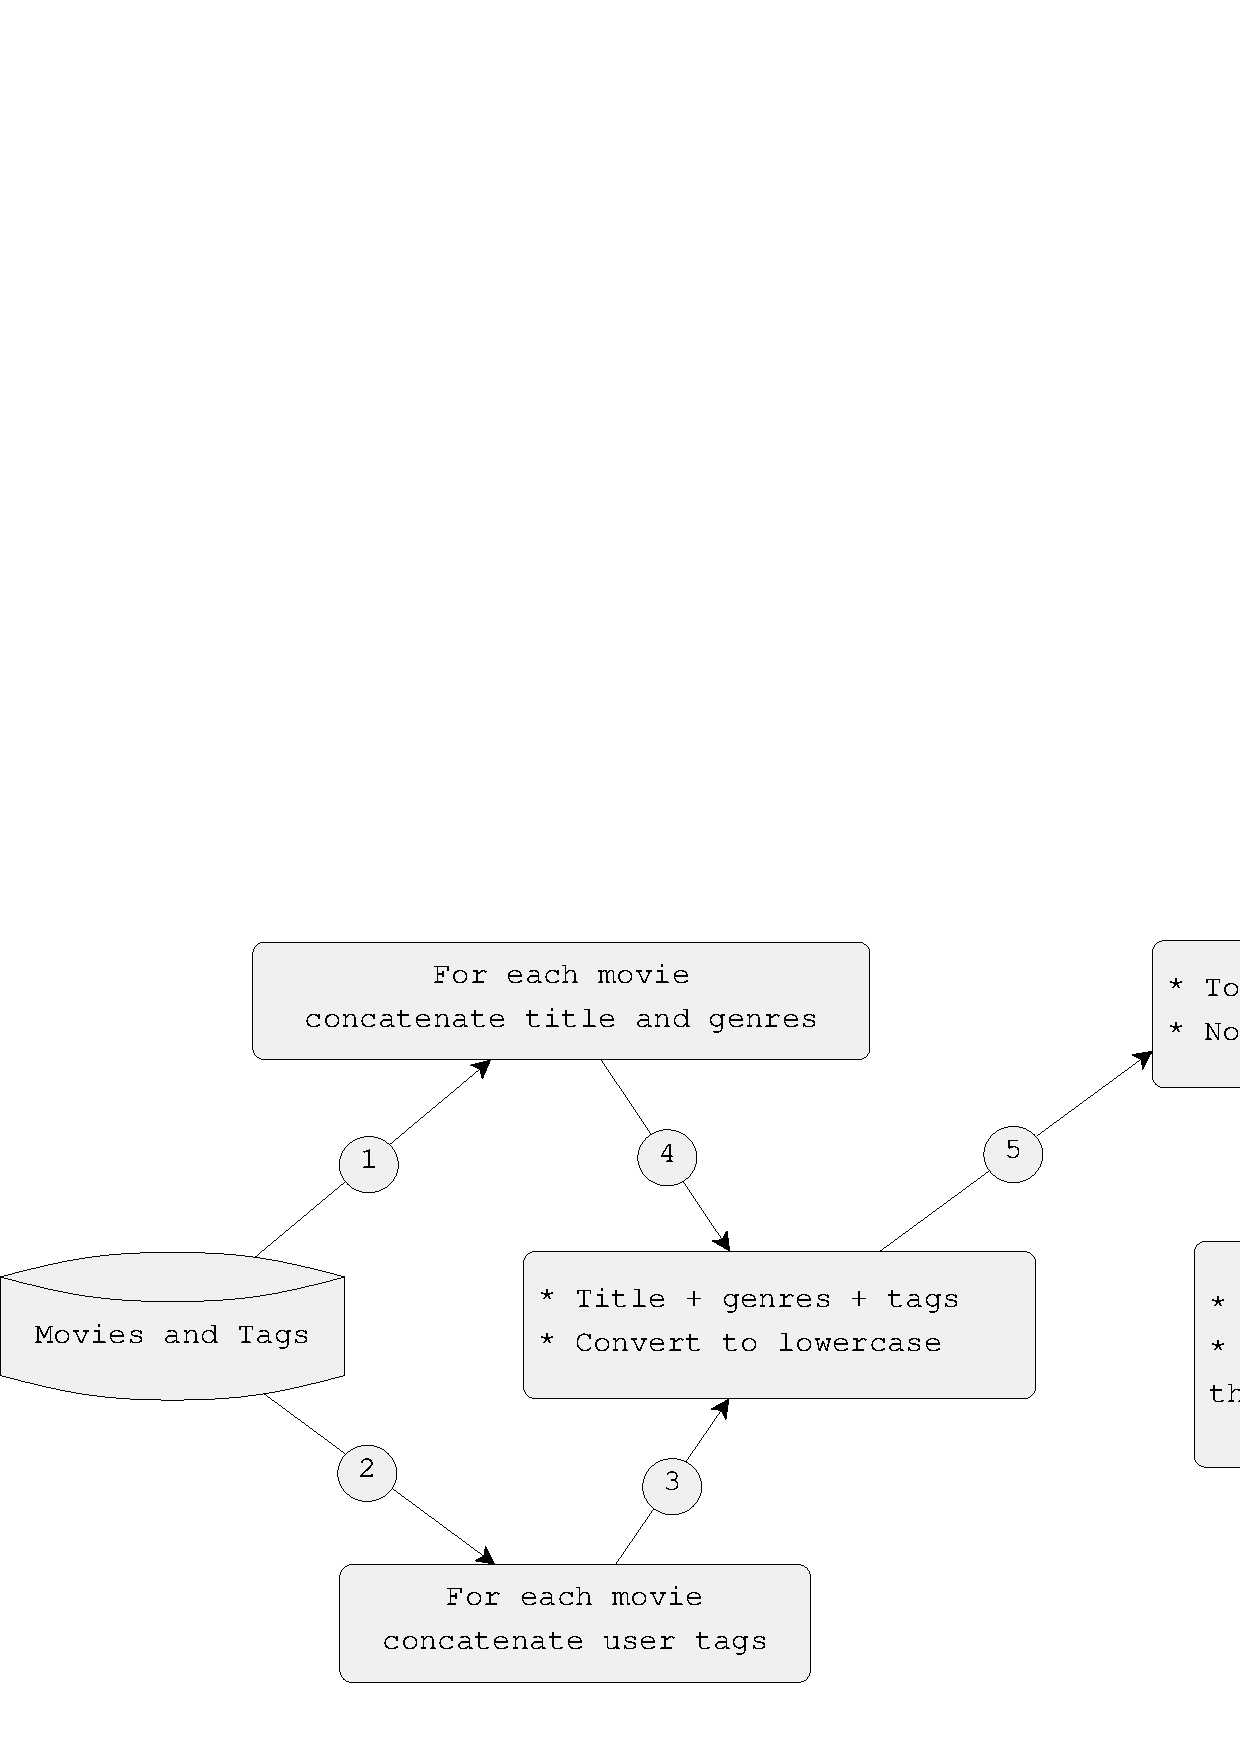
\includegraphics[width=\textwidth]{fig-003.pdf} %ativiUE.drawio.pdf
			\caption{Diagrama de atividades do fluxo esperado de emissão do voto.}
			\label{diagramaatividades}
			\source{Autor.}
		\end{minipage}
	\end{figure}
	
	
	Observações: 
	\begin{itemize}
		\item O dispositivo de coleta de dados biométricos tanto no cadastro quanto no momento da votação também deve ser íntegro, podendo ser submetido a um outro algoritmo de validação;
		\item Com os dados biométricos registrados na rede, o eleitor seria capaz de votar de qualquer UE da rede;
		\item Este modelo de votação poderia ser aplicado em uma votação remota e online, com o auxílio de um dispositivo móvel capaz de verificar biometria com precisão. Se isso ocorresse, contribuiria de fato para atingir o princípio da generalidade (\Cref{requisitos-eleicao}), mas não garantiria a incoercibilidade por meio de terceiros.
	\end{itemize}
	
	Com este modelo de \textit{E-Voting} é possível contribuir com a discussão acerca da confiabilidade do processo eleitoral brasileiro uma vez que é atacado o principal ponto de crítica do sistema atual. No sistema atual, a falta de confiabilidade baseia-se na premissa que a UE atual não é concordante com o princípio da independência de software, uma vez que sua execução depende do software e hardware embarcados. No modelo proposto, o contrato inteligente é público antes, durante e depois do período de eleição. Além disso, no modelo atual, a apuração dos votos também é contestada, e no modelo proposto, por se tratar de uma rede não permissionada para consulta de votos, a apuração também seria pública e auditável por quem desejar.
	
	
	
	\subsubsection{Contrato inteligente}\label{exemplo-contrato}
	
	Durante o \textit{design} do modelo, foi desenvolvido um contrato inteligente para servir de apoio ao modelo apresentado. 
	A rede \emph{blockchain} utilizada durante o desenvolvimento do projeto foi a \emph{Ethereum}, escolhida por sua popularidade e pela boa disponibilidade de escrever contratos inteligentes numa linguagem de alto nível, a \textit{Solidity}.  Um dos pontos da escolha foi a facilidade de implantação destes contratos \cite{dannen2017introducing}. Para isso, o ambiente de testes escolhido foi a IDE (\textit{Integrated Development Environment}) \textit{online} do \textit{Remix Project}. Nesta plataforma, foi possível escrever o contrato, compilar, realizar o \textit{deploy} e executar as transações de teste. 
	
	Durante a escrita do contrato, inicialmente foram definidas as estrutura de dados e as variáveis auxiliares, as quais podem ser vistas na \Cref{Codigo-estruturas}. As estruturas criadas foram "Voto'' e "Candidato''. Tendo essas estruturas, foram definidos "\emph{mappings}''. Esta estrutura de dados funciona como os dicionários (chave-valor) de outras linguagens de programação. Os \textit{mappings} foram criados para armazenar "candidatos'', "votos'', "eleitores'', "eleitoresVotantes'' e "votosPorCadidato''. Além disso, foi definido o contador de votos "totalVotos'', as definições do horário de início e fim da votação, e um evento de "votoEmitido''. 
	
	%Solidity language
	%\definecolor{verylightgray}{rgb}{.97,.97,.97}
	
	\lstdefinelanguage{Solidity}{
		keywords=[1]{anonymous, assembly, assert, balance, break, call, callcode, case, catch, class, constant, continue, constructor, contract, debugger, default, delegatecall, delete, do, else, emit, event, experimental, export, external, false, finally, for, function, gas, if, implements, import, in, indexed, instanceof, interface, internal, is, length, library, log0, log1, log2, log3, log4, memory, modifier, new, payable, pragma, private, protected, public, pure, push, require, return, returns, revert, selfdestruct, send, solidity, storage, struct, suicide, super, switch, then, this, throw, transfer, true, try, typeof, using, value, view, while, with, addmod, ecrecover, keccak256, mulmod, ripemd160, sha256, sha3}, % generic keywords including crypto operations
		keywordstyle=[1]\color{blue}\bfseries,
		keywords=[2]{address, bool, byte, bytes, bytes1, bytes2, bytes3, bytes4, bytes5, bytes6, bytes7, bytes8, bytes9, bytes10, bytes11, bytes12, bytes13, bytes14, bytes15, bytes16, bytes17, bytes18, bytes19, bytes20, bytes21, bytes22, bytes23, bytes24, bytes25, bytes26, bytes27, bytes28, bytes29, bytes30, bytes31, bytes32, enum, int, int8, int16, int24, int32, int40, int48, int56, int64, int72, int80, int88, int96, int104, int112, int120, int128, int136, int144, int152, int160, int168, int176, int184, int192, int200, int208, int216, int224, int232, int240, int248, int256, mapping, string, uint, uint8, uint16, uint24, uint32, uint40, uint48, uint56, uint64, uint72, uint80, uint88, uint96, uint104, uint112, uint120, uint128, uint136, uint144, uint152, uint160, uint168, uint176, uint184, uint192, uint200, uint208, uint216, uint224, uint232, uint240, uint248, uint256, var, void, ether, finney, szabo, wei, days, hours, minutes, seconds, weeks, years},	% types; money and time units
		keywordstyle=[2]\color{teal}\bfseries,
		keywords=[3]{block, blockhash, coinbase, difficulty, gaslimit, number, timestamp, msg, data, gas, sender, sig, value, now, tx, gasprice, origin},	% environment variables
		keywordstyle=[3]\color{violet}\bfseries,
		identifierstyle=\color{black},
		sensitive=true,
		comment=[l]{//},
		morecomment=[s]{/*}{*/},
		commentstyle=\color{gray}\ttfamily,
		stringstyle=\color{red}\ttfamily,
		morestring=[b]',
		morestring=[b]"
	}
	
	
	
\begin{lstlisting}[language=Solidity, label=Codigo-estruturas, caption={Contrato Inteligente desenvolvido utilizando Solidity.}, source={Autor.}]
pragma solidity ^0.8.0;

contract SistemaEleitoral {
	
	//Estrutura do voto
	struct Voto {
		address eleitor;
		int candidatoId;
	}
	
	//Candidatos participantes da eleicao
	struct Candidato {
		string NomeCandidato;
		string UrlFotoCandidato;
		string NomeVice;
		string UrlFotoVice;
		int Numero;
	}
	
	//Dicionario de eleitores
	mapping(string => bool) eleitores;
	
	//Dicionario de eleitores que votaram
	mapping(string => bool) eleitoresVotantes;
	
	//Dicionario de candidatos
	mapping(int => Candidato) candidatos;
	
	//Dicionario de votos
	mapping(uint => Voto) votos;
	
	//Numero de votos por candidato
	mapping(int => int) private votosPorCandidato;
	
	
	uint public totalVotos;
	
	//Hora do inicio da votacao
	uint public horaMinimadeVotos = 1664708400;
	
	//Hora do encerramento da votacao
	uint public horaMaximadeVotos = 1664740800;
	
	//Evento para notificar emissao de voto
	event VotoEmitido (address eleitor, int candidatoId);
}
\end{lstlisting} %stopzone
	
	
	%Talvez remover
	%A estrutura "\textbf{Voto}'' é uma estrutura composta pelo endereço de rede da UE e o identificador do candidato. A estrutura "\textbf{Candidato}'' é composta pelas informações do candidato, como seu número de identificador, seu nome, as informações de seu vice (se aplicável), e o endereço da URL da imagem com intuito de exibição na UE semelhante ao modelo atual. O mapeamento da linha 21 define uma lista "\textbf{eleitores}'' que armazena os dados dos eleitores, através de seu dado de identificação única. No exemplo foi utilizado um dado do tipo \textit{string}, entretanto, em um caso real poderia ser outro tipo, dependendo do tipo de autenticação escolhida. A lista "\textbf{eleitoresVotantes}'' inicia o período de eleição vazia, e a partir do momento que o eleitor registra seu voto, tem sua identificação armazenada nesta estrutura. A lista "\textbf{candidatos}'' armazena objetos do tipo "\textbf{Candidato}''. A lista "\textbf{votos}'' armazena objetos do tipo "\textbf{Voto}''. A lista "\textbf{votosPorCandidato}'' mapeia o número de votos que cada candidato recebeu, sendo atualizada a cada voto. O contador "\textbf{totalVotos}'' armazena o número de votos, sendo atualizada a cada voto. A variáveis "\textbf{horaMinimadeVotos}'' e "\textbf{horaMaximadeVotos}'' armazenam no formato \textit{Unix TimeStamp} os horário pré-definidos para o início e fim do período de votação. Neste exemplo, foi definido utilizando os horário de votação do primeiro turno das eleição para Presidente de 2022 em 2 de Outubro, que ocorreu das 08 horas até as 17 horas no horário de Brasília. Por fim, o evento "\textbf{votoEmitido}'' é um evento para ser disparado a cada voto.
	
	Na \Cref{Codigo-registroeleitres} foram definidas as funções para registro de eleitores e candidatos. Estas funções são de uso antes da eleição e são de responsabilidade da autoridade eleitoral responsável (atualmente seriam o TSE e os TREs).
	
	
	%Solidity language
\begin{lstlisting}[language=Solidity, label=Codigo-registroeleitres, caption={Funções para registrar candidatos e eleitores.}, source={Autor.}]
function registrarCandidato(string memory NomeCandidato, string memory UrlFotoCandidato, string memory NomeVice, string memory UrlFotoVice, int Numero) public {
	uint horaAtual = obterHoraAtual();
	require(horaAtual < horaMinimadeVotos, "Candidatos nao podem ser registrados durante ou depois da eleicao.");
	candidatos[Numero] = Candidato(NomeCandidato, UrlFotoCandidato, NomeVice, UrlFotoVice, Numero);
	votosPorCandidato[Numero] = 0;
}

function registrarEleitor(string memory eleitor) public {
	uint horaAtual = obterHoraAtual();
	require(horaAtual < horaMinimadeVotos, "Eleitores nao podem ser registrados durante ou depois da eleicao.");
	eleitores[eleitor] = true;
}	
\end{lstlisting} %stopzone
	
	No \autoref{Codigo-registroeleitres}, o método \textbf{registrarCandidato} (linha 2) recebe como parâmetro dados de um candidato apto a disputar a eleição e registra no \textit{mapping} candidatos e votosPorCandidato. Estas informações são seu número único, e nome e endereço da imagem do candidato e seu vice. Este método verifica se esta na fase 1 da eleição. 
	Similarmente, o método \textbf{registrarEleitor} (linha 10), recebe como parâmetro dados do eleitor. Neste caso é apenas uma \textit{string}, mas num caso real seria o \textit{hash} de alguma informação biométrica ou coisa do tipo. Verifica se está na fase 1 e registra que existe este eleitor no \textit{mapping} eleitores. Na \autoref{Codigo-auxiliar} foi definida a função \textit{obterHoraAtual} para obter a hora atual na rede em formato \textit{Unix TimeStamp}.
	
	
%Solidity language
\begin{lstlisting}[language=Solidity, label=Codigo-auxiliar, caption={Função auxiliar para obter hora atual em Unix TimeStamp do Contrato Inteligente desenvolvido.}, source={Autor.}]
function obterHoraAtual() public view returns (uint) {
	return block.timestamp; 
}
\end{lstlisting} %stopzone
	
	Na \autoref{Codigo-voto} está definida a função principal de registro de voto. Esta função recebe como parâmetro a identificação do eleitor e o número do candidato a ser votado. A partir disso, são feitas verificações para garantir que o voto a ser emitido é valido. Nas linhas 6, 9 e 12, é verificado se o precedimento está dentro do período de votação, se o eleitor é válido e se o eleitor já votou, respectivamente. Validado isso, o código verifica a existência ou não do candidato escolhido. Vale ressaltar, que para atender o princípio da capacidade do voto inválido (\Cref{requisitos-eleicao}), o sistema deve registrar votos inválidos ou nulos. Por isso, se o número do candidato não for encontrado, este é considerado um voto inválido, e é registrado com o número -1. Entretanto, para tratar o voto em branco, foi considerado o número fixo aleatório pré-definido, que associado  como um "candidato'' previamente cadastrado, e tem seu voto armazenado. 
	Feito isso, o contexto inicia os processos de registro do voto: registrar o voto propriamente dito na lista "\textbf{votos}'', somar o voto na estrutura "\textbf{votosPorCandidato}'', marcar o eleitor como votante na estrutura "\textbf{eleitoresVotantes}'', somar mais um voto no contador de votos e por fim emitir o evento "\textbf{VotoEmitido}''.
	
%Solidity language
\begin{lstlisting}[language=Solidity, label=Codigo-voto, caption={Método para registrar o voto do Contrato Inteligente desenvolvido utilizando Solidity.}, source={Autor.}]
// Registra um novo voto
function emitirVoto(int candidatoId, string memory eleitorId) public {
	uint horaAtual = obterHoraAtual();
	
	// Verifica se esta em periodo de eleicao
	require(horaAtual >= horaMinimadeVotos && horaAtual < horaMaximadeVotos, "Votos nao podem ser registrados fora do periodo de eleicao.");
	
	// Verifica se o eleitor esta registrado
	require(eleitores[eleitorId], "Somente eleitores registrados podem votar.");
	
	// Verifica se o eleitor ja votou
	require(!eleitoresVotantes[eleitorId], "Eleitores podem votar apenas uma vez.");
	
	// Verifica se o candidato nao esta registrado
	if (candidatos[candidatoId].Numero == 0){
		// Adiciona o voto na contagem de votos nulos
		votosPorCandidato[-1]++;
		// Registra o voto
		votos[totalVotos] = Voto(msg.sender, -1);
	}
	else {
		// Adiciona o voto na contagem do candidato (inclui o candidato "Branco")
		votosPorCandidato[candidatoId]++;
		// Registra o voto
		votos[totalVotos] = Voto(msg.sender, candidatoId);
	}
	
	// Armazena o eleitor na lista de eleitores votantes
	eleitoresVotantes[eleitorId] = true;
	
	// Incrementa o contador de votos
	totalVotos++;
	
	// Emite um evento de registro do voto
	emit VotoEmitido(msg.sender, candidatoId);
}
\end{lstlisting} %stopzone
	
	
	
	Por fim, na \Cref{Codigo-consultas} foram definidas as funções de consulta para candidatos e votos. As funções de candidatos buscam através de seu número de identificação e as funções de votos retornam o total de votos em um número bruto ou para cada candidato. Ambas as funções de consulta de voto respeitam o período final da eleição. 
	
%Solidity language
\begin{lstlisting}[language=Solidity, label=Codigo-consultas, caption={Funções de consulta do Contrato Inteligente.}, source={Autor.}]
// Obter Candidato
function getCandidato(int candidatoId) public view returns (Candidato memory) {
	return candidatos[candidatoId];
}

// Retorna o total de votos registrados
function getTotalVotos() public view returns (uint) {
	uint horaAtual = obterHoraAtual();
	
	// Verifica se o periodo de eleicao esta encerrado
	require(horaAtual >= horaMaximadeVotos, "A contagem de votos pode ser exibida apenas apos o periodo de eleicao.");
	
	return totalVotos;
}

// Total de votos registrados para cada candidato
function getVotosCandidato(int candidatoId) public view returns (int) {
	uint horaAtual = obterHoraAtual();
	
	// Verifica se o periodo de eleicao esta encerrado
	require(horaAtual >= horaMaximadeVotos, "A contagem de votos pode ser exibida apenas apos o periodo de eleicao.");
	
	return votosPorCandidato[candidatoId];
}
\end{lstlisting} %stopzone
	
	Algumas considerações sobre este modelo são que propositalmente que informações dos votos foram armazenadas de maneiras diferentes e redundantes com o intuito de poder trazer ainda mais uma camada de transparência e auditoria, uma vez que o valor de "\textbf{TotalVotos}'' deve ser igual a quantidade de objetos do tipo "\textbf{voto}''  na lista "\textbf{votos}'', que deve ser igual a soma dos valores da lista "\textbf{votosPorCandidato}'', que por sua vez deve ser igual ao número de itens na lista "\textbf{eleitoresVotantes}''. Embora o teste tenha sido realizado apenas com um nó, foi possível trocar as opções de servidores e executar algumas vezes as transações. Dessa forma, o plano da execução do contrato está contido na \Cref{execuçaocontarto}.
	
	%Com estas informações e com o contrato escrito, para o cenário de experimentação foi utilizada a plataforma \textit{Remix} para compilar e executar o contrato. Foi escolhido um ambiente virtual grátis do próprio \textit{Remix}, e por essa razão os testes foram executados apenas na plataforma.
	
	
	
	\begin{table}[htbp]
		\centering
		\caption{Passos da execução do contrato inteligente.}
		\label{execuçaocontarto}
		\newcolumntype{Y}{>{\raggedright\arraybackslash}X}
		\begin{tabularx}{\textwidth}{YYY}
			\toprule
			\textbf{Passo} & \textbf{Ação}  & \textbf{Descrição} \\
			\midrule
			Passo 1 & Preparação do ambiente & Corresponde a Fase 1 do processo. O contrato, contendo o horário atualizado do período de votação foi compilado e publicado na \textit{Remix VM}.\\
			\midrule
			Passo 2 & Cadastro de Informações & Ainda durante a Fase 1 do processo, foram registrados dados de eleitores e candidatos. Também foi testado o registro e consulta de votos fora do período. \\
			\midrule
			Passo 3 & Registro de votos & Iniciada a Fase 2, os votos foram registrados de maneira aleatória, contendo apenas um voto nulo. Foram testados o registro de candidatos e eleitores e a consulta de votos fora de período. \\
			\midrule
			Passo 4 & Consulta de votos & Iniciada a Fase 3, os votos foram consultados e foram testados o registro de eleitores e candidatos e a emissão de votos fora do período de votação. \\
			\bottomrule
		\end{tabularx}
		\source{Autor.}
	\end{table} 
	
	
	A implantação do contrato foi feita em um ambiente virtual (\Cref{deploy}) e o acesso do contrato na região de contratos publicados (\Cref{contratos}). Com o contrato acessível via interface, foi permitido executar as transações e funções especificadas, sendo possível cadastrar eleitores e candidatos, votar e verificar a cobertura das restrições, como não votar mais de uma vez e respeitar os períodos de votação para votar e consultar votos. % Note nas Figuras 10-18 alguns resultados do teste realizado.
	Na \Cref{deploy}, é possível observar a área de \textit{deploy} da plataforma \textit{Remix}, onde é possível selecionar o ambiente da publicação, neste caso a \textit{Remix VM} de \textit{Shanghai}, a conta, definir o limite de \textit{gas} e valores. Neste local é possível também selecionar o contrato a ser publicado, sendo que este deve ser compilado pelo \textit{Remix}.
	Na \Cref{contratos}, é possível acompanhar a listagem de transações possíveis com o contrato publicado. Esta lista é gerada automaticamente pelo \textit{Remix} após a publicação do contrato. Nessa listagem é possível preencher parâmetros e executar as transações.
	
	
	\begin{figure}[htbp]
		\centering
		\begin{minipage}{0.5\textwidth}
			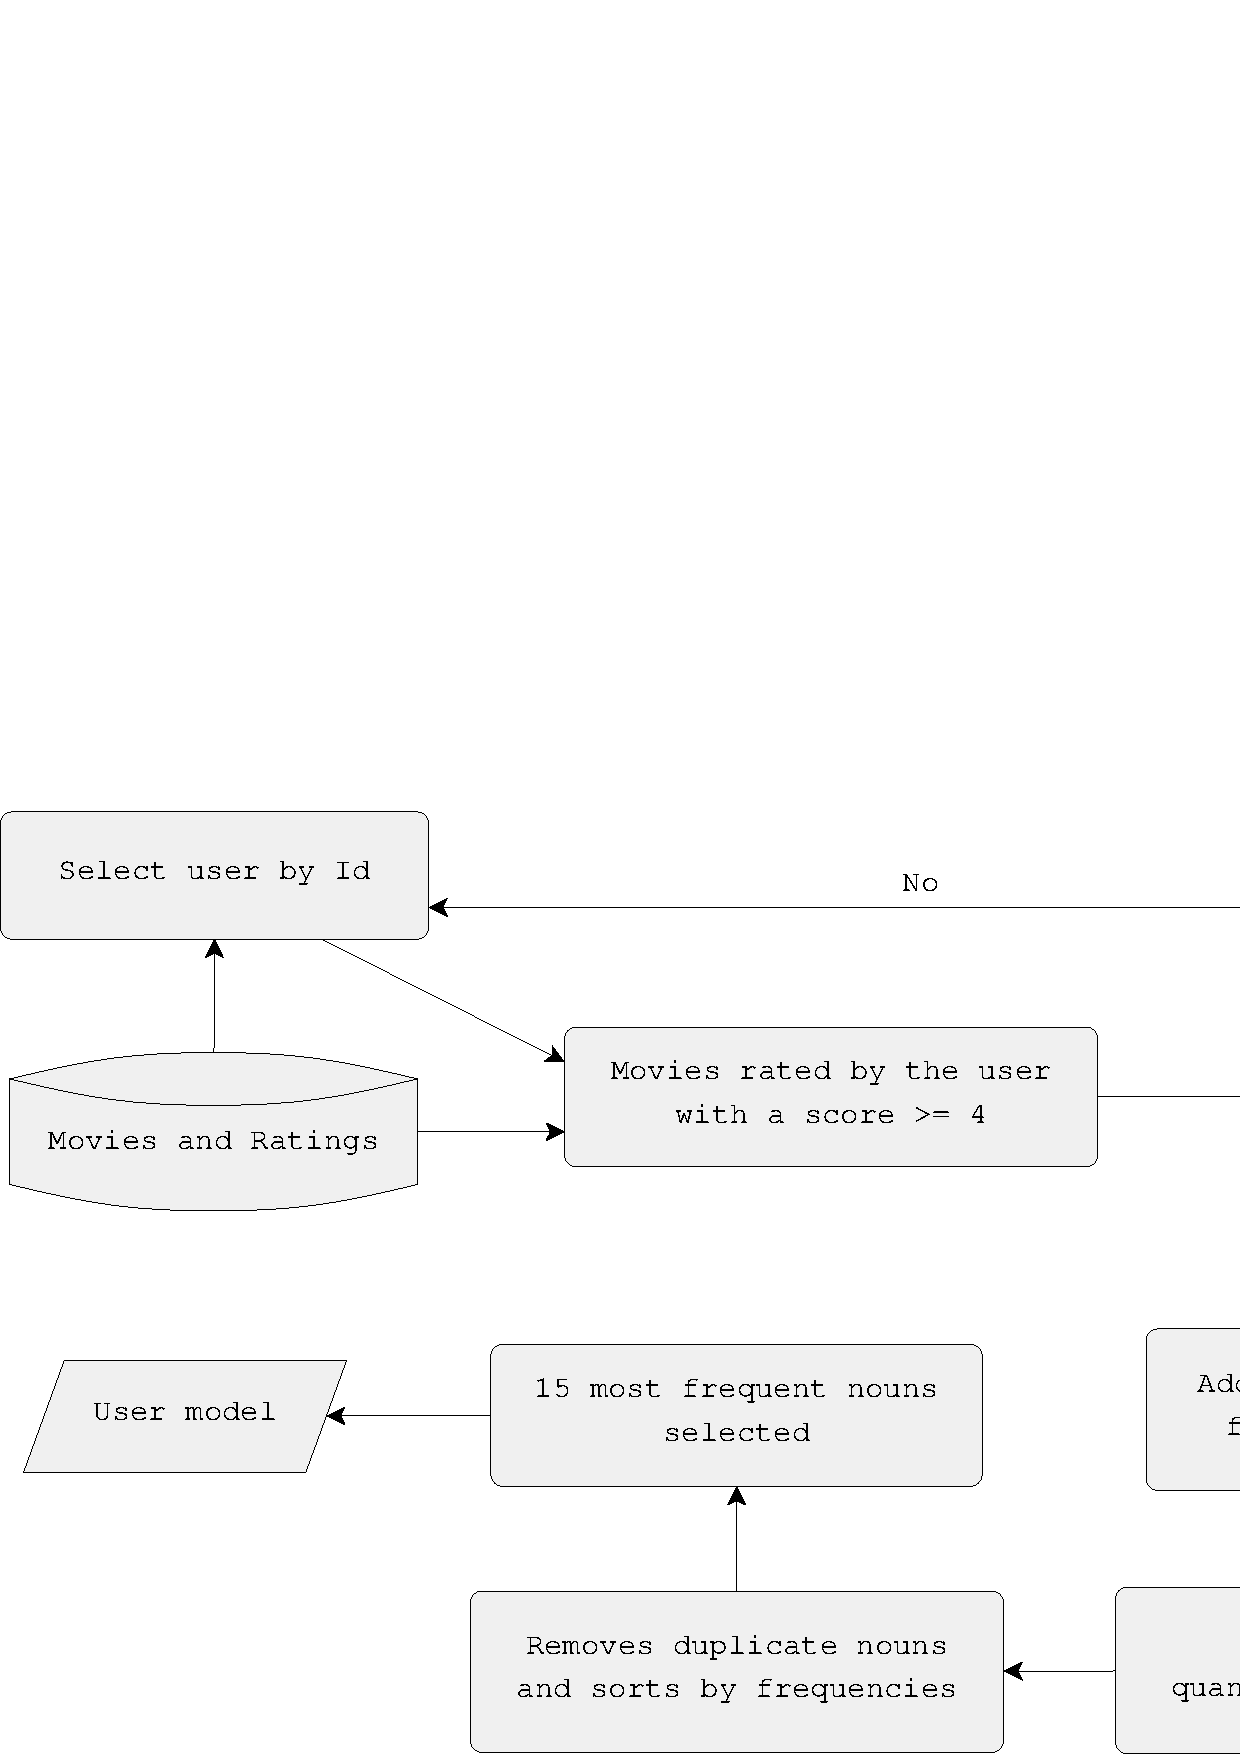
\includegraphics[width=\textwidth]{fig-004.png} %deploy.png
			\caption{Área de \textit{deploy} do \textit{Remix}.}
			\label{deploy}
			\source{Autor.}
		\end{minipage}
	\end{figure}
	
	
	
	
	\begin{figure}[htbp]
		\centering
		\begin{minipage}{.5\textwidth}
			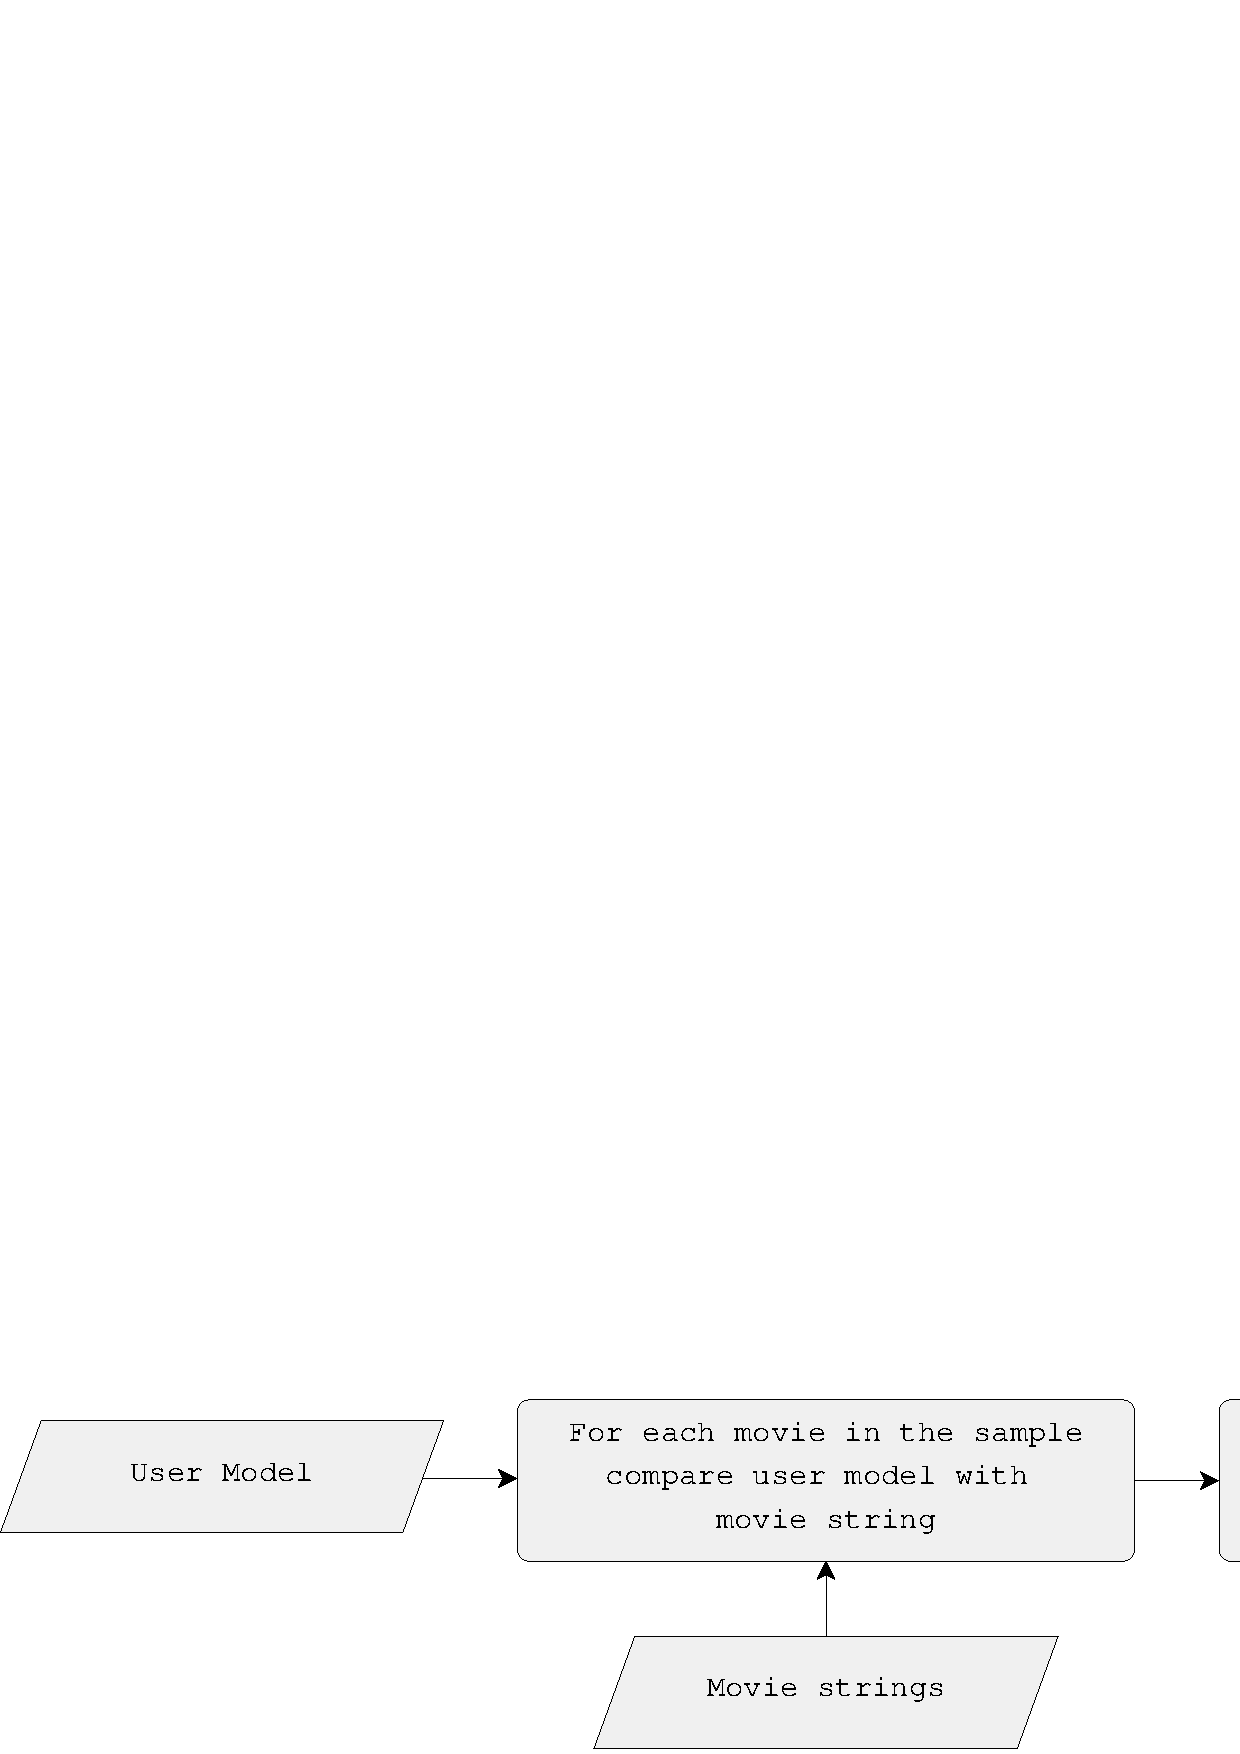
\includegraphics[width=\textwidth]{fig-005.png} %contract.png
			\caption{Transações disponíveis na área de contratos publicados.}
			\label{contratos}
			\source{Autor.}
		\end{minipage}
	\end{figure}
	
	
	
	\begin{figure}[htbp]
		\centering
		\begin{minipage}{1\textwidth}
			\includegraphics[width=\textwidth]{fig-006.png} %Testes/1registroeleitor.png
			\caption{Execução da transação de registrar eleitor.}
			\label{dash-transa}
			\source{Autor.}
		\end{minipage}
	\end{figure}
	
	Na \Cref{dash-transa} é possível notar o status, informações e o resultado da transação. Neste caso, foi executa uma transação de registra eleitor. O mesmo acontece na \autoref{registracandidato}, que mostra a execução de uma transação de registrar um candidato, com destaque para as informações referentes a transação como o \textit{hash}, custo, entrada e saída de dados. A \Cref{transacoes} mostra o acompanhamento de algumas dessas transações realizadas.
	
	
	\begin{figure}[htbp]
		\centering
		\begin{minipage}{1\textwidth}
			\includegraphics[width=\textwidth]{fig-007.png} %Testes/2registro de candidato.png
			\caption{Execução da transação de registrar candidato.}
			\label{registracandidato}
			\source{Autor.}
		\end{minipage}
	\end{figure}
	
	\begin{figure}[htbp]
		\centering
		\begin{minipage}{1\textwidth}
			\includegraphics[width=\textwidth]{fig-008.png} %Testes/3registro de eleitores e candidatos antes do horario.png
			\caption{Acompanhamento da execução das transações.}
			\label{transacoes}
			\source{Autor.}
		\end{minipage}
	\end{figure}
	
	\begin{figure}[htbp]
		\centering
		\begin{minipage}{1\textwidth}
			\includegraphics[width=\textwidth]{fig-009.png} %Testes/5emitir_voto.png
			\caption{Execução da transação de emitir voto.}
			\label{emitirvoto}
			\source{Autor.}
		\end{minipage}
	\end{figure}
	
	A \Cref{emitirvoto} mostra a execução da transação de emitir um voto. Na direita, é possível notar os parâmetros dos identificadores do candidato e do eleitor, sendo enviados. Na parte parte maior da imagem pode-se acompanhar o resultado da transação.
	
	Já a \Cref{obtencaodevotos} mostra outra parte importante do processo que é a obtenção de votos. Neste caso, na área direita foi submetida a transação para obter a quantidade de votos do candidato com identificador "1", e na janela de saída é possível ver o resultado, que mostra a contagem de 4 votos.
	
	
	\begin{figure}[htbp]
		\centering
		\begin{minipage}{1\textwidth}
			\includegraphics[width=\textwidth]{fig-010.png} %Testes/8obtencaodevotos.png
			\caption{Obtenção de votos por candidato durante a fase 3.}
			\label{obtencaodevotos}
			\source{Autor.}
		\end{minipage}
	\end{figure}
	
	Um dos pontos importantes da utilização destes contratos é a automação das regras de negócio e consequentemente, das restrições. Nas \Cref{failregistro}, \Cref{failemitirvotomaisdeumavez} e \Cref{failtentativadevotos} é mostrado a manutenção da restrição de não poder registrar eleitores ou candidatos durante o período de votação, de um eleitor não poder registrar um voto mais de uma vez e a tentativa de obtenção de resultados antes do fim do período de votação. Na plataforma é possível acompanhar as transações que foram rejeitadas, assim como o motivo, neste caso, disparado pelo contrato.
	
	\begin{figure}[htbp]
		\centering
		\begin{minipage}{1\textwidth}
			\includegraphics[width=\textwidth]{fig-011.png} %Testes/4naopoderegistraraposinicio.png
			\caption{Tentativas de cadastrar eleitores ou candidatos após o início sendo rejeitadas.}
			\label{failregistro}
			\source{Autor.}
		\end{minipage}
	\end{figure}
	
	\begin{figure}[htbp]
		\centering
		\begin{minipage}{1\textwidth}
			\includegraphics[width=\textwidth]{fig-012.png} %Testes/7tentativa de voto com o mesmo identificador de eleitor.png
			\caption{Tentativa rejeitada de votar mais de uma vez com o mesmo identificador de eleitor.}
			\label{failemitirvotomaisdeumavez}
			\source{Autor.}
		\end{minipage}
	\end{figure}
	
	
	\begin{figure}[htbp]
		\centering
		\begin{minipage}{1\textwidth}
			\includegraphics[width=\textwidth]{fig-013.png} %Testes/97tentativa de obter votos antes do fim da eleição
			\caption{Tentativa rejeitada de obter quantidade de votos antes da fase 3.}
			\label{failtentativadevotos}
			\source{Autor.}
		\end{minipage}
	\end{figure}
	
	\begin{figure}[htbp]
		\centering
		\begin{minipage}{1\textwidth}
			\includegraphics[width=\textwidth]{fig-014.png} %Testes/10votos nulos.png
			\caption{Obtenção de votos nulos, representado pelo identificador -1.}
			\label{votosnulos}
			\source{Autor.}
		\end{minipage}
	\end{figure}
	
	Por fim, a \Cref{votosnulos} mostra a obtenção de votos nulos, também de suma importância neste tipo de votação, sendo representados pelo indicador -1, que no caso de testes foi submetido apenas uma vez. 
	
	Após a bateria de testes, pode-se concluir que cumpriu a expectativa da regra de negócio proposta, uma vez que com o contrato público, foi possível realizar as transações de acordo com as regras. Entretanto,  por limitações, não foi possível garantir requisitos quanto segurança e resiliência.
	
	Um fato interessante a se relatar após a execução dos testes é que o consumo de algumas transações podem consumir valores de \textit{gas} relativamente altos. Embora os testes tenham sido realizados em um ambiente virtual grátis, é possível observar a quantidade de \textit{gas} consumidos durante a transação. Em alguns casos, a transação chegou a consumir aproximadamente U\$ 0,25, o que tornaria uma possível aplicação real num contexto de eleições nacionais bem custoso, pois ao multiplicar pela quantidade de votos da eleição de 2022 resultaria numa quantia perto de R\$ 150 milhões. Entretanto, há a possibilidade de executar o sistema em uma rede própria com o objetivo de reduzir o custo.
	
	
	\subsection{Desafios Jurídicos e Políticos}
	A implementação de tecnologias emergentes em eleições nacionais não envolve apenas desafios técnicos, mas também uma série de barreiras jurídicas e políticas. A legislação eleitoral brasileira teria que ser revisada para acomodar o uso de blockchain e contratos inteligentes, principalmente no que diz respeito à segurança do voto e à privacidade dos eleitores. A adoção de uma infraestrutura descentralizada levanta questões sobre quem teria a autoridade final para auditar e validar os resultados eleitorais.
	
	Políticos e eleitores também podem ser resistentes à mudança, principalmente em um contexto onde o sistema eleitoral atual, baseado em urnas eletrônicas, é amplamente aceito, mas também alvo de questionamentos. A transparência oferecida pelo blockchain poderia resolver alguns problemas de confiança no processo, mas sua implementação prática dependeria de uma regulamentação clara e de um consenso político amplo, o que pode ser difícil de alcançar.
	
	Além disso, jurisprudência internacional sobre o uso de blockchain em eleições ainda é escassa, embora iniciativas como o E-Estônia forneçam um ponto de partida para estudos comparativos. O debate sobre a aplicabilidade e a segurança de eleições baseadas em blockchain está em andamento, com defensores apontando suas vantagens em termos de transparência e adversários destacando a complexidade de regular tecnologias descentralizadas em cenários eleitorais críticos.

	\section{Conclusão \label{conclusao}}
	
	
	Este trabalho propôs um modelo de estrutura de votação eletrônica que pode ser aplicado em e-voting e com necessidade de garantir os requisitos de um sistema seguro, transparente e íntegro, como o cenário das eleições nacionais. Evidentemente este se trata de um trabalho inicial, não refletindo uma solução finalizada para aplicação  em um cenário real. Este trabalho contribui com discussões recentes a cerca da confiabilidade das Urnas Eletrônicas do tipo DRE (\textit{Direct Recording Eletronic}), propondo um modelo descentralizado com uma transparência, segurança e auditabilidade adicional, através do uso de contratos inteligentes em redes \textit{blockchain} públicas.
	
	%Foi realizada uma pesquisa de busca exploratória nas bases de dados para obter os problemas e motivos que geraram a discussão atual, assim como os conceitos de rede distribuída, votação eletrônica e os trabalhos relacionados a esta temática. Essas informações foram dispostas nos Capítulos \ref{trabalhosRelacionados} e \ref{fundamentacaoteorica}. A partir destas pesquisas foi possível entender que grande parte da discussão parte do fato das UEs utilizadas serem de primeira geração, de possuírem brechas encontradas durante as sessões de Testes Públicos de Segurança e a possível parcialidade advinda de um controle absoluto de uma autoridade central. Foi possível encontrar também iniciativas promissoras que combinam votação eletrônica e redes descentralizadas. 
	
	Foram encontradas iniciativas que combinam votação eletrônica e redes descentralizadas. Diante disso, foi possível concluir que esta premissa era um campo de estudo inicial mas com grande potencial para trazer as características almejadas para a discussão. Assim, foi proposto um modelo para uso em eleições contando ainda com o recurso das seções presenciais de votação, mas com interligação das urnas para registro e consulta dos votos, sendo a consulta pública após o encerramento do período de votação. Foi descrito também um \textit{smart-contract} desenvolvido em Solidity e testado em ambiente \textit{Ethereum}.
	
	Para o uso deste modelo, evidentemente seria necessária uma complexidade maior de desenvolvimento, além é claro dos esforços necessários pelos órgãos competentes. Por se tratar de um contexto crítico, seu desenvolvimento deverá ser muito criterioso e transparente, para que sua confiabilidade seja aceita. %Entretanto, por este desenvolvimento ser centralizado e a tomada de decisão do modelo a ser utilizado ser concentrada, potencialmente sempre existirá alguma desconfiança nestes processos.
	Para trabalhos futuros, sugere-se o desenvolvimento do produto, com mais blocos descentralizados e maior atenção aos conceitos de criptografia entre estes blocos, além de testes de viabilidade, segurança e integridade destes possíveis sistemas descentralizados.
	
	\printbibliography\label{sec-bib}
	% if the text is not in Portuguese, it might be necessary to use the code below instead to print the correct ABNT abbreviations [s.n.], [s.l.]
	%\begin{portuguese}
	%\printbibliography[title={Bibliography}]
	%\end{portuguese}
	
	%full list: conceptualization,datacuration,formalanalysis,funding,investigation,methodology,projadm,resources,software,supervision,validation,visualization,writing,review
	\begin{contributors}[sec-contributors]
		\authorcontribution{José Alves de Lima Neto}[conceptualization,datacuration,investigation,methodology,software,validation,writing,review]
		\authorcontribution{Rafael Oliveira Vasconcelos}[methodology,projadm,supervision,resources,validation,writing,review]
	\end{contributors}
	
	
\end{document}

